%%%%%%%%%%%%%%%%%%%%%%%%%%%%%%%%%%%%%%%%%%%%%%%%%%%%%%%%%%%%%%%%%%%%%%%%%%%%%%%%
%2345678901234567890123456789012345678901234567890123456789012345678901234567890
%        1         2         3         4         5         6         7         8

%\documentclass[letterpaper, 10 pt, conference]{ieeeconf}  % Comment this line out
                                                          % if you need a4paper


\documentclass[a4paper, 10pt, conference]{ieeeconf}      % Use this line for a4
                                     \usepackage[normalem]{ulem}                     % paper

\IEEEoverridecommandlockouts                              % This command is only
                                                          % needed if you want to
                                                          % use the \thanks command
\overrideIEEEmargins
% See the \addtolength command later in the file to balance the column lengths
% on the last page of the document


% !TEX root = ../main.tex
% !TeX encoding = UTF-8
\usepackage{verbatim}
%\usepackage[portuguese]{babel}
%\usepackage[brazilian]{babel}
%\usepackage[brazilian]{babel}
\usepackage[utf8]{inputenc}
\usepackage[T1]{fontenc}


\usepackage{todonotes}
%\usepackage[algoruled,linesnumbered,lined,portuguese]{algorithm2e}
\usepackage[algoruled,linesnumbered,lined]{algorithm2e}



\usepackage{tabularx}
\newcolumntype{L}[1]{>{\raggedright\arraybackslash}p{#1}}
\newcolumntype{C}[1]{>{\centering\arraybackslash}p{#1}}
\newcolumntype{R}[1]{>{\raggedleft\arraybackslash}p{#1}}

% *** CITATION PACKAGES ***
\usepackage{cite}


% *** GRAPHICS RELATED PACKAGES ***
%\usepackage[pdftex]{graphicx}

% *** MATH PACKAGES ***
\usepackage{amsmath}
\usepackage{amssymb}
\usepackage{amstext}
\usepackage{amscd}
%\usepackage{amsthm}


% *** PDF, URL AND HYPERLINK PACKAGES ***
\usepackage{url}

% correct bad hyphenation here
\hyphenation{op-tical net-works semi-conduc-tor}

%
%
\usepackage{tabularx,dcolumn} %tabela
\usepackage{booktabs}
\newcommand{\raaa}[1]{\renewcommand{\arraystretch}{#1}}

\newcommand{\vars}{\texttt}
\newcommand{\func}{\textrm}


\newcommand{\hardware }{\textit{hardware}}
\newcommand{\Hardware }{\textit{Hardware}}
\newcommand{\software }{\textit{software}}
\newcommand{\Software }{\textit{Software}}
\newcommand{\hardwares}{\textit{hardwares}}
\newcommand{\Hardwares}{\textit{Hardwares}}
\newcommand{\softwares}{\textit{softwares}}
\newcommand{\Softwares}{\textit{Softwares}}

\newcommand{\hs}{\textit{hardware}\ e\ \textit{software}}
\newcommand{\HS}{\textit{Hardware}\ e\ \textit{Software}}

\newcommand{\wearable} {\textit{wearable}}
\newcommand{\Wearable} {\textit{Wearable}}
\newcommand{\wearables}{\textit{wearables}}
\newcommand{\Wearables}{\textit{Wearables}}


\newcommand{\lut}      {\textit{Lookup Table}}
\newcommand{\ff}       {\textit{Flip Flop}}
\newcommand{\luts}     {\textit{Lookup Tables}}
\newcommand{\ffs}      {\textit{Flip Flops}}
\newcommand{\buffer}   {\textit{buffer}}
\newcommand{\design}   {\textit{design}}
\newcommand{\designer} {\textit{designer}}
\newcommand{\Design}   {\textit{Design}}
\newcommand{\Designer} {\textit{Designer}}
\newcommand{\designs}  {\textit{designs}}
\newcommand{\designers}{\textit{designsers}}
\newcommand{\Designs}  {\textit{Designs}}
\newcommand{\Designers}{\textit{Designers}}
\newcommand{\assembly} {\textit{assembly}}
\newcommand{\profile}  {\textit{profile}}
\newcommand{\Profile}  {\textit{Profile}}
\newcommand{\speedup}  {\textit{speedup}}
\newcommand{\Speedup}  {\textit{Speedup}}
\newcommand{\core}     {\textit{core}}
\newcommand{\cores}    {\textit{cores}}
\newcommand{\codesign} {\textit{codesign}}
\newcommand{\mobile}   {\textit{mobile}}
\newcommand{\benchmark}   {\textit{benchmark}}
\newcommand{\benchmarks}   {\textit{benchmarks}}
\newcommand{\Benchmark}   {\textit{Benchmark}}
\newcommand{\Benchmarks}   {\textit{Benchmarks}}
\newcommand{\titulo}{Uma Abordagem do Problema de Particionamento \Hardware\ e \Software\ para \Design\ de Sistemas Computacionais \Wearables}

\newcommand{\A}{$\mathcal{A}$}
\newcommand{\B}{$\mathcal{B}$}
\newcommand{\C}{$\mathcal{C}$}
\newcommand{\Ss}{$\mathcal{S}$}
\newcommand{\R}{$\mathcal{R}$}

%Hyphenations
\hyphenation{XHSTT}
%\hyphenation{res-tri-ções}
\hyphenation{co-nhe-ci-do}
\hyphenation{co-nhe-ci-da}
\hyphenation{re-a-li-za}
\hyphenation{vi-zi-nho}
\hyphenation{clim-bing}
\hyphenation{ran-king}
\hyphenation{me-lhor}
\hyphenation{ou-tras}
\hyphenation{ge-ra-das}
\hyphenation{ex-pe-ri-men-tos}
\hyphenation{pro-ble-ma}
%\hyphenation{su-ges-tões}
\hyphenation{pos-te-rior-men-te}


\title{\LARGE \bf
An Approach of Hardware and Software Partitioning for the Wearables Design with Limited Reconfigurable Hardware Resources
}

\author{ \parbox{6 in}{\centering Rodolfo Labiapari Mansur Guimarães and Ricardo Augusto Rabelo Oliveira \\
         %\thanks{*Use the $\backslash$thanks command to put information here}\\
         %Departamento de Ciência da Computação\\
         Department of Computer Science \\
         %Universidade Federal de Ouro Preto, Brasil\\
         Federal University of Ouro Preto \\
         {\tt\small rodolfolabiapari@decom.ufop.br, rrabelo@gmail.com}}
         %\hspace*{ 0.5 in}
         %\parbox{3 in}{\centering Dr. 
         %%\thanks{*Use the $\backslash$thanks command to put information here}\\
         %Departamento de Ciência da Computação\\
         %Universidade Federal de Ouro Preto\\
         %Ouro Preto, 35400--000, Brasil\\
         %{\tt\small rrabelo@gmail.com}}
}

\begin{document}


\maketitle
\thispagestyle{empty}
\pagestyle{empty}

% 200, 300 palavras
\begin{abstract}

%1) Contextualização: É a parte que está lá, onde vc passa a ideia geral da área.
%As tecnologias em microeletrônica, sensores e comunicação móvel têm sido constantemente melhoradas à medida que a informação torna-se mais necessária. 
%Tornam-se um estímulo para o desenvolvimento de sistemas inteligentes e conectados como sistemas embarcados, IoTs ou \wearables,\ visto pelo rápido desenvolvimento desses para o mercado.
%Entretanto ainda com a dificuldade de satisfazer os requisitos de aumento de desempenho e redução de consumo energético das várias aplicações autônomas modernas.
The technologies in microelectronic, sensors and mobile communication have been continuously improved as information becomes more needed.
They become a stimulus for the development of intelligent and connected systems as embedded systems, IoTs or wearables, seen by the rapid growth of theses for the market.
However, still with difficulty to satisfy the requirements of performance increase and reduction of the energy consumption of the various autonomous modern applications.
%Utilizam de um conjunto de sensores e necessitam de um serviço autônomo, o que implica numa demanda de desempenho somado com o baixo consumo de energia.
%
%2) Gap: O que ainda falta na área que foi contextualizada? (especificamente o problema no qual vc "toca").
%Análise de desempenho no uso de FPGA com particionamento em \hardware\ para sistemas embarcados têm sido fortemente abordada pela comunidade acadêmica. 
%Porém, não há pesquisas que abordam o problema de particionamento para sistemas \wearable.
Performance analysis in the use of FPGA with hardware partitioning for embedded systems has been strongly addressed by the academic community.
Also, there are not researches that address the partitioning problem for wearable systems.
%
%3) Propósito: O que o seu artigo faz? Que tipo de problema vc está endereçando?
%Este trabalho tem como objetivo o aprimoramento de desempenho de dispositivos computacionais \wearables\ em \hardwares\ reconfiguráveis, visando otimizações no uso de recursos e reduzindo o consumo energético%
This work has as objective the enhancement of performance of wearable computers devices in reconfigurable hardware, targeting optimizations in the use of resources and reducing the energy consumption
%
%4) Metodologia: O que vc utilizou no desenvolvimento do seu artigo. Deve ser curto.
%, utilizando particionamento \hs\ como meio.
, using hardware and software partitioning.
%
%5) Resultados: Qual foi o principal (ou os principais resultados) obtidos? 
%6) Conclusões: Qual a sua conclusão mais relevante?
%Os resultados mostram que é possível obter maior desempenho em sistemas \wearables\ utilizando plataforma FPGA apenas com a realocação de algoritmos candidatos em \hardware.
The results show that it is possible to obtain higher performance in wearable systems using FPGA platform only with the relocation of candidates algorithms in hardware.


Key-words: Hardware and Software Partitioning, Wearable System, FPGA, Performance.
\end{abstract}

% !TEX root = ../main.tex
% !TeX encoding = UTF-8
\section{Introduction} \label{chap:introducao}

    %\todo[inline]{1) Contextualização: Apresente uma visão da área identificando a importância do contexto q está trabalhando. Introduza os "termos" mais importantes.}
    
    %O projeto de Sistemas Embarcados (SE) está cada dia mais complexo \cite{Jozwiak2017}. 
    %
    %A demanda por curto tempo para disponibilidade de produtos ao mercado somado ao fato de exigirem propriedades como alto desempenho, baixo consumo de energia e alocação de recursos, representam um desafio para projetistas de sistemas \wearables.
    The demand for the short time for availability of products to the market summed up to the fact of requiring proprieties as high performance, low energy consumption and resources allocation, represent a challenge for wearable systems designers.
    
    % wearable
    %Sistemas \Wearables,\ uma subcategoria de Sistemas Embarcados (SE), possuem o propósito de integrar-se ao sistema corporal, expandindo suas capacidades, criando uma integração cada vez mais intensa entre tecnologia e ser humano.
    Wearable Systems, a subcategory of Embedded Systems (ES), have the propose of integrating to the body system, expanding its capabilities, making an integration each more intense between technology and human being.
    %
    %Esses sistemas possuem diversos componentes implementados em \hs\ e ainda é um desafio combinar alto desempenho com baixo consumo de energia maximizando o tempo de uso \cite{Wolf1994, Edwards1994}.
    These systems have several components implemented in hardware and software, and it is still challenging to combine high performance with low energy consumption, maximizing the use time \cite{Wolf1994, Edwards1994}.
    %
    %Uma das maneiras de lidar com tais problemas consiste na combinação das funções do processador com os recursos dos Arranjo de Portas Programáveis em Campo (FPGAs, do inglês \textit{Field-Programmable Gates Array}) formando um sistema computacional híbrido.
    One of the ways of dealing with such problems consists of the combination of the processor functions with the resources of Field-Programmable Gates Array (FPGA) forming a hybrid computational system.
    
    
    %particionamento
    %Uma decisão que pode ser tomada em nível de implementação nestes sistemas é chamado de Particionamento \HS\ (também abreviado como particionamento) e tem se mostrado promissor aumentando o desempenho destes sistemas \cite{Sass2010, BenHajHassine2017}.
    A decision that can be taken in implementation level in these systems it is called Hardware and Software Partitioning (also abbreviated as partitioning) and has shown promise increasing performance those systems \cite{Sass2010, BenHajHassine2017}.
    
    %\todo[inline]{3) Descreva o estado da arte atual, sempre referenciando trabalhos importantes.}
    
    %Alguns trabalhos mostram que, uma implementação customizada em \hardware\ pode prover maior eficiência energética e \speedup, comparado à implementações em \software\ \cite{Zhang2008, BenHajHassine2017, Wolf1994, Canis2011, Stone2010}.
    Some works show that a custom implementation in hardware can provide higher energy efficiency and speedup, comparing to implementations in software \cite{Zhang2008, BenHajHassine2017, Wolf1994, Canis2011, Stone2010}.
    %
    %Em \cite{Jozwiak2017} \todo{[VJP] essa referência está no contexto do seu trabalho? Ou ela somente fala de dipositivos móveis e vestíveis? Se for genérica, sugiro retirar essa frase.}  exibe-se vários estudos sobre dispositivos móveis e \wearables\ e \cite{Trindade2016} afirma que um significante esforço foi posto na área de particionamento de SE nos últimos dez anos.
    
    
    %\todo[inline]{2) Gap: Quais são as questões em aberto, restrições e limitações do estado atual dessa pesquisa.}
    
    %Entretanto, mesmo com vários estudos relacionados à desempenho com particionamento de SE em plataformas FPGA, não existem estudos que avaliam a melhoria de desempenho especificamente para \wearables\ em plataformas FPGA.
    However, even with various researches related to performance with ES partitioning in FPGA platforms, there are not researches that evaluate performance improvement especially for wearables in FPGA platforms.
    
    
    %\todo[inline]{4) Propósito+metodologia: Descreva o propósito do seu artigo utilizando para isso uma pitada da sua metodologia.}
    
    %Esta pesquisa consiste no particionamento de alguns algoritmos candidatos dentro do \wearable\ comparando o desempenho, alocação de recursos e gasto energético de ambas as implementações \hs.
    This research consists of the partitioning of some candidates algorithms inside of the wearable comparing the performance, resources allocated and energy spent on both hardware and software implementations.
    %
    % combinação de fpga com cpu
    %Ao utilizar o FPGA é possível implementar um sistema e acelerá-lo usando recursos de \hardware\ por meio do particionamento, o que melhora o desempenho e eficiência energética \cite{Cong2009, Lo2009, Zhang2008a}.
    Utilizing the FPGA it is possible to implement a system and speed it up using hardware resources by partitioning, that increase the performance and energy efficiency \cite{Cong2009, Lo2009, Zhang2008a}.
    
    
    %\subsection{Contribuição}
    %parece mais objetivo que contribuição
    %Esta pesquisa consiste numa busca sobre o aprimoramento de desempenho de dispositivos computacionais \wearables\ em \hardwares\ reconfiguráveis, utilizando particionamento \hs\ como meio.
    %Visa gastos relativos ao uso de recursos em \hardware\ e gasto energético.
    %A principal contribuição deste trabalho é exibir que particionamento \hs\ é uma excelente técnica para a melhoria de desempenho de sistemas \wearables,\ como será exibido.
    The main contribution of this work it is shown that hardware and software partitioning it is an excellent technique for the performance improvement of wearable systems, as will be explained.
    
    %Adicionalmente, algumas contribuições específicas são listadas a seguir:
    Additionally, some specifics contributions are listed below:
    
    \begin{enumerate}
        \item 
        %Apresentação da modelagem do problema de particionamento \hs\ aplicando tal técnica nessa classe de sistemas embarcados, buscando pelo aprimoramento de desempenho;
        
        %Apresentação de uma modelagem do problema de particionamento aplicado à \wearables,\ buscando maior desempenho;
        Presentation of modeling of partitioning problem applied to wearables, targeting higher performance;
        
        \item 
        % wearables e particionamento
        %Introdução de sistemas computacionais \wearables\ na qual possuem restrições de consumo energético e recursos, utilizando uma plataforma FPGA como meio para análise de recursos alocados; 
        %Utilização de plataforma FPGA em sistemas \wearables\ com restrições energéticas e de recursos;
        Utilization of FPGA platform in wearable systems with resources and energy restrictions;
        
        
        \item %Obtenção de pelo menos $9,6\%$ a mais de desempenho em três de quatros algoritmos avaliados, alocando $5,5\%$ de recursos de \hardware\ reconfigurável e aumento de $ 5,4\% $ de gasto energético;
        %Análise de desempenho de quatro algoritmos utilizando particionamento em \hardware\ considerando alocação de recursos e consumo energético;
        Performance analysis of four algorithms using partitioning in hardware considering resources allocated and energy spent;
        
        \item 
        %Análise de como as interfaces de comunicação entre \hs\ e otimizações influenciam no desempenho dos \wearables.
        Analyse of how the communication interfaces between hardware and software and optimizations influence in wearable performance.
        
        %\item Os resultados mostram que com o uso da técnica de particionamento \hs\ em pedaços de código do \wearable,\ aumentou-se o desempenho do sistema pelo menos 2,2\%, chegando até em 41,6\% a mais em desempenho.
    \end{enumerate}

    %Avaliou-se algoritmos do sistema \wearable\ analisando o desempenho e alocação de cada um, sendo eles o Estatístico \Ss$_{Es}$, Lagrange \Ss$_{La}$, Números Primos \Ss$_{NP}$ e Risco \Ss$_{Ri}$ e para cada um obteve-se uma melhora de desempenho em relação à sua versão em \software\ de 2,2\%, $41,6\%$, $9,6\%$ e $17,8\%$ respectivamente.
    We evaluated algorithms of wearable system analyzing the performance and allocation of each one, begin them the Statistic \Ss$_{Es}$, Lagrange \Ss$_{La}$, Prime Numbers \Ss$_{NP}$ and Risk \Ss$_{Ri}$ and for each one was obtained a performance enhance related to its version in software of 2,2\%, 41,6\%, 9,6\% and 17,8\% respectively.
    
%    As próximas seções foram divididas da seguinte forma: 
%    Seção \ref{chap:revisao_bibliografica} apresenta a informações relevantes para o compreendimento e os trabalhos relacionados. 
%    Seção \ref{chap:design} exibe a metodologia utilizada.
%    Seção \ref{chap:prototipo} descreve o protótipo e o procedimento de testes.
%    Seção \ref{chap:results} exibe e analisa os resultados e a Seção \ref{chap:conclu} conclui e apresenta os trabalhos futuros.
%    
    The following sections were divided in this way:
    Section \ref{chap:revisao_bibliografica} presents information relevant to the understanding and related work.
    Section \ref{chap:design} shows the methodology used.
    Section \ref{chap:prototipo} describes the prototype and test procedure.
    Section \ref{chap:results} displays and analyzes the results and Section \ref{chap:conclu} concludes and presents future work.
    

%!TEX root = ../main.tex
% !TeX encoding = UTF-8
\section{Wearables as Processing Systems} \label{chap:revisao_bibliografica}
   \subsection{Systems for Wearable Devices}
      % Introdução histórica e geral
      
      %Sistemas \wearables\ são sistemas que proporcionam ao usuário um nível superior de informações contextualizadas dentro de um ambiente interativo, tendo um computador acoplado ao corpo \cite{Amorim2017}.
      Wearable systems are systems that provide to the user a higher level of contextualized information inside of an interactive environment, having a computer coupled to the body \cite{Amorim2017}.

      %Devido ao movimento de seus usuários, um controlador/processador \wearable\ é embutido em um ambiente móvel e necessita da interação com o ambiente ao seu redor.
      %Esses SE podem também trabalhar de forma colaborativa com \textit{smartphones}, redes e outros sistemas, criando soluções mais complexas \cite{Jozwiak2017}.
      Due to the movement of the users, a wearable controller/processor is embedded in a mobile environment and needs of the interactions with the situation around.
      These ES can also work collaboratively with smartphones, networks and others systems, making solutions more complexes \cite{Jozwiak2017}.
      

      %A utilização de FPGA nos permite alcançar alto poder de processamento com eficiência energética para tarefas de computação intensiva em tempo real, por exemplo \cite{Plessl2003}.
      The FPGA utilization allows us to reach high processing power with energy efficiency for intensive computation tasks in real time, for example \cite{Plessl2003}.


   \subsection{Field-Programmable Logic Device (FPGA)}

      %LUTS
      %O FPGA, segundo \cite{tocci2003sistemas}, constitui-se de vários módulos lógicos pequenos, independentes, programáveis e interconectados para criar funções maiores.
      %É composto principalmente \ffs\ e de \luts,\ que podem ser de dois tipos \luts\ e \luts RAM.
      The FPGA, according to \cite{tocci2003sistemas}, constitutes of various little logic modules, independents, programmables and interconnected to create bigger functions.
      It composes mainly of Flip-Flops and Lookup Tables (LuTs), that can be in two types Lookup Tables and Lookup TablesRAM.
      
      %De acordo com a quantidade de recursos disponíveis por meio do FPGA é possível implementar inúmeros projetos digitais, como por exemplo, funções de processamento de imagem, algoritmos de redes de computadores, algoritmos criptográficos e \textit{soft}-processadores completos \cite{Plessl2003, Choi2016}.
      %Uma das principais formas de sintetização é utilizando Sintetização em Alto Nível (HLS, \textit{High Level Synthesis}).
      According to with the number of available resources of FPGA it is possible to implement many digitals projects, as for examples, image processing functions, algorithms of computer networks, cryptographic algorithms and soft-processors \cite{Plessl2003, Choi2016}.
      One of the main ways of synthetization is using High-Level Synthesis (HLS), where it is possible to create new hardware projects using high-level codification.

%!TEX root = ../main.tex
% !TeX encoding = UTF-8
\subsection{Related Works}  \label{chap:relacionados}
    
    %Em \cite{Mei2000} além do particionamento, os autores apresentam uma abordagem de escalonamento para SE dinamicamente reconfigurável (DRESs, do inglês \textit{dynamically reconfigurable embedded systems}). 
    %Neste trabalho os autores fornecem análises dos tempos de configuração e reconfiguração parcial do FPGA e mostram que o algoritmo proposto resolve o problema de particionamento e escalonamento dos DRES.
    In \cite{Mei2000} besides of the partitioning, the authors present a scheduling approach for the dynamically reconfigurable ES (DRES).
    In this work, they provide analysis of configuration and partial reconfiguration time of FPGA and show that the algorithm proposed to solve the partitioning and scheduling problem for DRESs.
    
    %Em \cite{Arato2003} os autores descrevem algumas versões do problema de particionamento para sistemas de tempo real e custo restringido, provando que são problemas $ \mathcal{NP} $-difícil.
    %Adicionalmente, apresentam uma abordagem com programação linear inteira, resolvendo o problema de forma otimizada, e uma abordagem utilizando algoritmo genético, na qual encontram-se soluções próximas ao ótimo global.
    In \cite{Arato2003} the authors describe some versions of the partitioning problem for real-time systems and restricted cost, proving that they are $ \mathcal{NP} $-hard problems.
    Additionally, present an approach with integer linear programming, solving the problem of optimal way, and an approach using the genetic algorithm, which found solutions near to the global optimum.
    
    %O trabalho em \cite{Mann2007} descreve uma primeira tentativa para um algoritmo exato para o problema de particionamento.
    %Utiliza um esquema no qual implementa-se a estratégia \textit{branch-and-bound} como um \textit{framework}.
    %Eles demonstram que problemas de particionamento altamente complexos podem ser resolvidos em tempo razoável.
    The work in \cite{Mann2007} describes the first try for an exact algorithm for the partitioning problem.
    It uses the scheme which implements the branch-and-bound strategy as a framework.
    They demonstrate that partitioning problems highly complex can be resolved in a reasonable time.
    
    
    %Pesquisas mais recentes, como a de \cite{BenHajHassine2017} procuram aplicar otimizações sobre o tempo de execução e gasto energético para processadores baseados em produtos embarcados, por meio de particionamento.
    %Comparado com outras heurísticas, o algoritmo mostra-se ser mais adequado para aplicações que necessitam do equilíbrio no \textit{tradeoff}.
    Researches more recent as the \cite{BenHajHassine2017} target to apply optimizations on execution time and energy spent on processors based in embedded products, by partitioning.
    Comparing with others heuristics, the algorithm show to be more suitable for applications that need of equilibrium in the tradeoff.
    
    %Trabalhos como o de \cite{Trindade2016} utilizam algoritmos genéticos para solucionar o problema de particionamento em SE.
    %Propõem novas abordagens usando técnicas de verificação baseadas nas teorias de módulo de satisfação (SMT, do inglês \textit{satisfiability modulo theories}).
    Works as the \cite{Trindade2016} use genetic algorithm to solve the partitioning problem of ES.
    Propose new approaches using techniques of verifications based on satisfiability modulo theories (SMT). 
    
    
    %concluindo tudo que foi dito
    %Os trabalhos citados buscam o estudo do desempenho e \design\ de SE no geral por meio de particionamento, mas nenhum com foco em \wearables.
    The cited works target the performance and design study of ES in general by partitioning, but none is aiming the wearables.
    
    
    %Em \cite{Jozwiak2017} os autores apresentam uma extensa revisão da literatura considerando vários aspectos de um SE, bem como suas tecnologias de \design,\ com foco em sistemas móveis modernos incluindo \wearables.
    In \cite{Jozwiak2017} the authors present an extensive revision of literature considering various aspects of an ES, as well as its technologies of design, aiming in mobile moderns systems including wearables.
    % wearable fpga
    %Além deste, é possível ver em \cite{Plessl2003, Ahola2007, Abdelhedi2016, Narumi2016, Lee2015} trabalhos que estudam \wearables\ junto de FPGA, mas nenhum deles utilizam a técnica de particionamento como meio para seu \design.
    Beside this, it is possible to see in \cite{Plessl2003, Ahola2007, Abdelhedi2016, Narumi2016, Lee2015} works that aim wearable with FPGA, but none uses the partitioning technique for its design.
    
    
    % conclusao
    %Este trabalho portanto consiste na análise do problema de particionamento \hs,\ com foco em \design\ de sistemas \wearables\ em plataforma FPGA.
    This work, therefore, consists in the analysis of hardware and software partitioning problem, with the focus in wearable systems design in FPGA platforms.


%!TEX root = ../main.tex
% !TeX encoding = UTF-8
\section{Principles of Partitioning of General Systems} \label{chap:design}
    
    %A seguir serão descritos tópicos utilizados para o entendimento do particionamento, seguindo conceitos estabelecidos por vários trabalhos como \cite{Arato2003, Arato2005, Mann2007, BenHajHassine2017, Sass2010}.
    %Esses tópicos são necessários para o entendimento básico dos arcabouços metodológicos de \codesign\ e o seu particionamento para sistemas, em especial para \wearables, além de definições formais sobre.
    Next will be described topics used to the knowledge of partitioning, following concepts established by various works as \cite{Arato2003, Arato2005, Mann2007, BenHajHassine2017, Sass2010}.
    These topics are necessary for the fundamental understanding of the codesign methodological frameworks and its partitioning for systems, in particular for wearables, besides formal definitions.
    
    %É possível descrever sistemas livre de especificações formais por meio de descrições de protótipos simples, conhecidos como \Design\ de Referência de \Software\ (DRS)\cite{Sass2010}.
    %Dessa forma, o algoritmo a ser analisado também pode ser representado como grafo de rotinas, chamado de Grafo de Controle de Fluxo (GCF) \cite{Mann2007}.
    %Ele é definido por $C = (B, F) \label{eq:subrotinaa}$
    %onde $B$ são vértices que representam as tarefas 
    %%http://www.dcc.ufrj.br/~gabriel/microarq/Escalonamento.pdf
    %e $ F $ são arestas que indicam todas as possibilidades de caminhos entre elas.
    It is possible to describe systems free of formal specifications by simple prototype descriptions, known as software reference design (SRD) \cite{Sass2010}.
    In this way, the algorithm to be analyzed also can be represented by a routing graph, called Control Flow Graph (CFG) \cite{Mann2007}.
    It is defined by $C = (B, F) \label{eq:subrotina}$ where $B$ are vertices that represent the tasks and $ F $ are edges that represent all the possibility of the path between them.
    
    
    %A decomposição de um DRS pode gerar dois componentes: uma porção a ser realizada em \hardware\ e outra executada em \software.
    %Essa decisão de divisão é chamada de Problema de Particionamento.
    The decomposition of a SRD can generate two components: a portion to be executed in hardware and other in software.
    This division decision it is called of Problem of Partitioning Hardware and Software.
    
    \subsection{Formal Definition of the Hardware and Software Partitioning Problem} \label{sec:gc}
        %Um Grafo de Chamada (GC) consiste num conjunto de GCFs, um por sub-rotinas, ou seja, $\mathcal{C} = {C_0, C_1, \dots C_{n-1}}$
        A Call Graph (CG) consists in a conjunct of CFGs, one by subroutines, that is, $\mathcal{C} = {C_0, C_1, \dots C_{n-1}}$
        %onde $ C_i = (B_i, F_i) $ representa o GCF de uma sub-rotina $ i $.
        where $ C_i = (B_i, F_i) $ represents the CFG of one subroutine $ i $.
        %Sendo assim, o grafo estático de chamada da aplicação completa é escrito por $\mathcal{A} = (\mathcal{C}, \mathcal{L}) \label{eq:aa}$
        Therefore, the static call graph of all application is describes by $\mathcal{A} = (\mathcal{C}, \mathcal{L}) \label{eq:a}$
        %onde \A\ representa uma aplicação específica e $ \mathcal{L} \subseteq \mathcal{C} \times \mathcal{C} $ é um subconjunto do plano cartesiano\footnote{Duas sub-rotinas são relacionadas se podem ser determinadas que, no tempo de compilação, a sub-rotina $ i $ tem potencial de invocar a sub-rotina $ j $, ou seja, $ (C_i, C_j) \in \mathcal{L} $.} dos GCFs.
        where \A\ represents an specific application and $ \mathcal{L} \subseteq \mathcal{C} \times \mathcal{C} $ is a subset of cartesian plan\footnote{Two subroutines are related if it can be determined that, at compile time, the subroutine $ i $ has the potential to invoke the subroutine $ j $, that is, $ (C_i, C_j) \in \mathcal{L} $.}
        of CFGs.
        
        
        %Com esses conceitos definidos, é possível definir-se também uma partição como $ \mathcal{S} = \{S_0, S_1, \dots S_i\} $ sendo $ i $ quantidade de partições, e $U$ como o conjunto de todas as sub-rotinas.
        %Assim, uma partição \Ss\ de um conjunto universal $ U $ é definida como um conjunto de subconjuntos de $ U $, podendo ser definida como
        With these concepts defined, it is possible to define also a partition as $ \mathcal{S} = \{S_0, S_1, \dots S_i\} $ being $ i $ the quantity of partitions, and $ U $ as the set of all the subroutines.
        Thus, a partition \Ss\ of a universal set a $ U $ is defined as a set of subsets of $ U $, can be described as
        %
        \begin{eqnarray}
        \bigcup_{S \in \mathcal{S}} S &=& U           \label{eq:part_form_1} \\
        \forall S, S' \in \mathcal{S} | S \cap S' &=& \emptyset  \label{eq:part_form_2}\\
        \forall S \in \mathcal{S}\ |\ S &\neq& \emptyset  \label{eq:part_form_3}
        \end{eqnarray}
        %
        %onde a Equação~\ref{eq:part_form_1} diz que cada elemento de $ U $ é um membro de pelo menos um subconjunto $ S \in \mathcal{S} $, e as Equações~\ref{eq:part_form_2} e \ref{eq:part_form_3} dizem que os subconjuntos $ S \in \mathcal{S} $ são emparelhados, disjuntos e não vazios.
        %Em outras palavras, cada elemento do nosso universo $ U $ termina exatamente em um dos subconjuntos de $\mathcal{S}$ e nenhum dos subconjuntos são vazios.
        where the Equation~\ref{eq:part_form_1} says that each element of $ U $ is a member at least one subset $ S \in \mathcal{S} $, and the Equations~\ref{eq:part_form_2} and \ref{eq:part_form_3} say that the subsets $ S \in \mathcal{S} $ are paired, disjoint and non-empty.
        In others words, each element of our universe $ U $ ends precisely in one of the subsets \Ss\ and none of the subsets are empty.
        
        %Com isso, é possível aplicar o formalismo à $ \mathcal{A} $, se assumirmos que nosso universo é o conjunto de todas as tarefas $B$ de um dispositivo \wearable\ e, assim, $U$ são as partições de sub-rotinas
        With that, it is possible to apply the formalism to \A,\ if we assume that our universe is the set of all the tasks $ B $ of a wearable device and so, $ U $ are the partitions of subroutines.
        %
        \begin{equation}
        U = \bigcup_{C \in \mathcal{C}} B(C) \label{eq:bigcup}
        \end{equation}
        %
        %sendo esta a partição natural da aplicação, onde
        being this the natural partition of the application, where
        %
        \begin{equation} \small
        \mathcal{S}  = \left \{
        \underbrace{\left \{ b_0, b_1, \dots b_{i-1} \right \}}_{\textnormal{subroutine }C_0},
        \underbrace{\left \{ b_i, b_{i+1}, \dots \right \}}_{\textnormal{subroutine }C_1},\dots
        \underbrace{\left \{ b_j, b_{j+1}, \dots \right \}}_{\textnormal{subroutine }C_{n-1}}
        \right \}
        \end{equation}
        
        
        \makeatletter
        \def\@eqnnum{{\normalsize \normalcolor (\theequation)}}
        \makeatother
        
        %
        %O propósito é a reorganização de $U$ em um particionamento com dois subconjuntos  $ \mathcal{S} = \{S_0, S_1\} $, sendo eles \hs.
        %Dessa forma, teremos uma nova partição \Ss$'$ gerando um novo resultado $ \mathcal{A}’ = (\mathcal{C}’, \mathcal{L}’) $, inferido a partir da reorganização da partição $ \mathcal{S} $.
        The propose is the reorganization of $ U $ in a partitioning with two subsets $ \mathcal{S} = \{S_0, S_1\} $, being them hardware and software.
        Therefore, we will have a new partition \Ss$ ' $ generating a new result $ \mathcal{A}’ = (\mathcal{C}’, \mathcal{L}’) $, inferred by partition reorganization \Ss.
        
        %O segundo passo é mapear cada subconjunto de $ \mathcal{S}' $ para ambos \hs,\ como é exibido na Equação \ref{eq:part_final}.
        The second step is to map each subset of \Ss$ ' $ for both hardware and software, as is shown in Equation \ref{eq:part_final}.
        
        { \small
        \begin{equation}
        \mathcal{S}'\!=\!\left \{
        \underbrace{
        \underbrace{
        \left \{ b_0, b_1, ... b_{i-1} \right \}
        }_{\textnormal{subroutine }C_0},
        ...
        \underbrace{
        \left \{ b_j, b_{j+1}, ... \right \}
        }_{\textnormal{subroutine }C_{n-i}}
        ...
        }_{\textnormal{software}};
        \ 
        \underbrace{
        \underbrace{
        \left \{ b_i, b_{i+1}, ... \right \}
        }_{\textnormal{subroutine }C_{n-1}}
        ...
        }_{\textnormal{hardware}}
        \right \} \label{eq:part_final}
        \end{equation}
        }
        
    
    
    \subsection{Performance as Guide to the Hardware and Software Partitioning} \label{sec:ganho_performance}
        \subsubsection{Performance Gain}
        
            %Para aplicações em geral pode estar no acúmulo de pequenos ganhos.
            %Entretanto, diferente de algoritmos em \software\ no qual tem-se análise de ordem de complexidade, em \hardware\ não possui-se um guia geral para comparação.
            For applications, in general, the gain can be in the accumulation of small profits.
            However, different of software level algorithms which have time complexity analysis, in hardware level have not a general guide for comparing.
            
            
            % y é speedup
            %O ganho, ao comparar uma solução \hs\ contra uma solução puramente \software,\ é tipicamente mensurado por meio do \speedup, e pode ser obtido utilizando a Equação~\ref{eq:speedup1}.
            %Utiliza-se $ \gamma $ para sua representação, permitindo comparar recursos diferentes para determinar melhores particionamentos.
            The gain, when comparing a hardware and software solution against an only software solution is typically measured by speedup, and it can be obtained using the Equation~\ref{eq:speedup1}.
            It uses $ \gamma $ for its representation, allowing to compare different resources to determine betters partitionings.
            %
            \begin{equation}
            \gamma =
            \frac{
            \textnormal{\textit{hardware speed}}
            }{
            \textnormal{\textit{software speed}}
            }
            =
            \frac{
            \frac{
            1
            } {
            \textnormal{\textit{hardware time}}
            }
            } {
            \frac{
            1
            }{
            \textnormal{\textit{software time}}
            }
            }
            =
            \frac{
            \textnormal{\textit{software time}}
            } {
            \textnormal{\textit{hardware time}}
            } \label{eq:speedup1}
            \end{equation}
            %
            %Mais especificamente, interessa-se no ganho de desempenho individual de cada recurso que pode ser definido como $ \gamma(i), i \in \mathcal{C}\ |\ \gamma(i) =\ ^s\!/_h $.
            %Para que um algoritmo em \hardware\ seja mais performático, deseja-se que $\gamma > 1$.
            Specifically, it interest in the individual performance gain of each resource that can be defined as $ \gamma(i), i \in \mathcal{C}\ |\ \gamma(i) =\ ^s\!/_h $.
            For an algorithm in hardware be more performative, it is desired that $ \gamma > 1 $.
            
        
        \subsubsection{Finite Resources in Electronic Components} \label{sec:recursos}
        
            %Um FPGA terá um valor escalar total $ r_{FPGA} $, que representa o total de números de \luts\ disponíveis para sintetização.
            %Então $ r(i) $ pode ser usado para representar a quantidade de recursos requerida por cada algoritmo $ i $.
            %Fazendo uma simples relação, tem-se que $ \sum_{i \in \mathbb{D}} r(i) < r_{FPGA} $ restringe quão largo $ \mathbb{D} $ pode crescer, onde $ \mathbb{D} $ é o conjunto de algoritmos candidatos.
            A FPGA will have a scalar value total $ r_{FPGA} $, that represents the total available of Lookup Tables for synthetization.
            So, $ r(i) $ can be used to represent the number of resources required for each algorithm $ i $.
            Making a simple relation, we has that $ \sum_{i \in \mathbb{D}} r(i) < r_{FPGA} $ restricts how large $ \mathbb{D} $ can grow, where $ \mathbb{D} $ is the set of candidates algorithms.
            
            %Uma típica plataforma FPGA moderna tem múltiplos tipos de recursos além de \luts,\ como memória, blocos DSP, etc., sendo a quantidade de recursos de cada tecnologia representados matematicamente por  $r_{Logic\ Cells}$, $r_{Memory}$, $r_{DSP}$, $r_{n-1} $, respectivamente.
            %Dessa forma, podem ser representados por um vetor de recursos
            A typical modern FPGA platform has multiples types of resources besides Lookup Tables, as memory, DSP blocks, etc., being the number of resources of each technology represent mathematically by $r_{Logic\ Cells}$, $r_{Memory}$, $r_{DSP}$, $r_{n-1} $, respectively.
            So, they can be represented by a resource vector
            %
            %$ \vec{r}_{FPGA} = (r_{Logic\ Cells}, r_{Memory}, r_{DSP}, \dots r_{n-1} ) $
            %
            
                     \begin{equation} \footnotesize 
                        \vec{r}_{FPGA} =
                        \begin{pmatrix}
                        r_{Logic\ Cells} \\
                        r_{Memory}\\
                        r_{DSP}\\
                        \vdots \\
                        r_{n-1}
                        \end{pmatrix}
                     \end{equation}
            
            %e com isso,
            and with that,
            %
            %\begin{equation}
            $\sum_{i \in \mathbb{D}} \vec{r}(i) < \vec{r}_{FPGA}$.
            %\end{equation}
            %
    
    
    \subsection{Wearable's Evaluation}
        %\todo[inline]{ explicando como a teoria da secao III se aplica na pratica ao seu experimento.} 
        
        %Enquanto o desempenho do \wearable\ é avaliada pelo tempo de execução do sistema segundo a Equação~\ref{eq:speedup1}, a alocação de recursos deve ser analisada, 
        %tanto em cada um dos \hardwares\ dos algoritmos gerados por HLS, quanto para o sistema como um todo, respeitando o limite de recursos $ \vec{r}_{FPGA}$.
        While system runtime evaluates the wearable's performance according to Equation~\ref{eq:speedup1}, the resources allocation must be analyzed, both in each of the hardware of the algorithms generated by HLS and for the system as a whole, respecting the resource limit $ \vec{r}_{FPGA}$.
        
        %Dessa forma, será utilizado \A$_{i}$\ para descrever separadamente as implementações dos $i$ códigos candidatos e \Ss$_{j}$\ referencia-se às implementações dos $j$ sistemas sintetizados.
        %
        %Com a diferenciação entre \A$_{i}$\ e \Ss$_{j}$\ (parte e todo do sistema)\ é possível analisar tanto as implementações dos módulos gerados por HLS separadamente, quanto os sistemas finais na alocação de recursos.
        So, it will be used \A$_{i}$\ to describe separately the implementations of the candidate codes $ i $ and \Ss$_{j}$\ to reference the implementations of the synthesized systems $ j $.
        With the differentiation between \A$_{i}$\ and \Ss$_{j}$\ (part and all of the system), \ is possible to analyze both the implementations of the HLS modules separately and the final systems in resource allocation.
        
        

%%!TEX root = ../main.tex
% !TeX encoding = UTF-8
%\chapter{O Particionamento de \HS\ para Sistemas \Wearables} \label{chap:desenvolvimento}
   \section{O Particionamento de Hardware e Software para Sistemas Wearables} \label{sec:desenvolvimento}

      %De início, será considerado como aplicaçãåo \wearable\ um conjunto de instruções organizadas, e como visto na Seção \ref{sec:gc}, esta também representada por uma coleção de grafos de controle de fluxo, ou seja, GC, especificando a sua ordem de execução.
      A partir deste, será feito análises a fim da procura de um particionamento que atenda aos requisitos de dispositivos \wearables\ como poder de processamento sem o \textit{trade-off} de energia, além de miniaturização, confiabilidade e outros.

      %Após esclarecidos algumas definições prévias (Seção~\ref{sec:definicoes_previas}), será apresentado o problema na Seção~\ref{sec:declaracao_problema}.
      %Alguns fatores podem ajudar nas decisões de particionamento tal como expectativa de ganho de performance (Seção \ref{sec:ganho_performance}) e os recursos utilizados em \hardware\ (Seção \ref{sec:recursos}).%, a forma na qual são usados e, talvez os mais importantes, quanto de sobrecarga de comunicação a decomposição impõe (Seção \ref{sec:comunicacao}) \todo{deixar?}e dificuldade de implementar um conjunto específico em \hardware\ (Seção \ref{sec:dificuldades}).\todo{organizar}


   \subsection{Declaração do Problema} \label{sec:declaracao_problema}
      %Nesta seção serão apresentadas as declarações matemáticas do problema de agrupamento de instruções em recursos e seus mapeamentos em \hardware\ ou \software, ou seja, o particionamento \hs.
      %Segundo \cite{Sass2010}, a forma mais comum de transcrever é descrever manualmente o \core\ com um HDL utilizando \design\ referencial de \software\ como especificação, método utilizado para descrever o problema.

      No particionamento, muitos problemas práticos impactam diretamente na performance do sistema.
      Nem todos os problemas podem ser incorporados num modelo analítico \cite{Wang2016}, e por isso, só podemos esperar que as soluções matemáticas produzam uma resposta aproximada ao problema de particionamento ao utilizar a declaração formal, pois muitas das entradas do modelo são estimadas ou aproximações no qual futuramente degrada a fidelidade de resultados.
      %%Este é um fato relevante pois com isso, resolvendo o problema de particionamento `no papel', tem-se um particionamento que é próximo ao ótimo.
      %%Assim, cabe ao \designer\ ser habilidoso em usar os guias e projetar uma solução mais refinada.
      Dessa forma, é mais eficiente usar uma combinação de técnicas \textit{ad hoc} e matemáticas para encontrar uma solução ótima ou aproximada como será feito, do que simplesmente confiar numa intuição.


      %\begin{comment}
      %\subsection{Declaração do Problema}
      %Já descrito as ferramentas matemáticas necessárias para descrever o problema fundamental do particionamento no Capítulo \ref{chap:revisao_bibliografica}, pode-se então descrever formalmente o problema em termos de variáveis. % e descrever um algoritmo \todo{algorit?}para encontrar uma solução aproximada.
      %
      %A ideia básica consiste em encontrar um particionamento para todos os blocos básicos de uma aplicação e então separá-los em \hs.
      Formalmente, procura-se por uma partição $ \mathcal{P} $ de todas as tarefas $ U $ de uma aplicação.
      %
      %$$ U = \bigcup_{C \in \mathcal{C}} B(C) $$
      %
      %$ C = (B,F) $
      Definida a partição e o universo, tem-se então um subconjunto $ \mathbb{C}\ |\ \mathbb{C} \subseteq U $, onde $ C \in \mathcal{C} $ é um vértice de um $ \mathcal{A} = (\mathcal{C}, \mathcal{L}) $.
      O conjunto $ \mathbb{C} $, chamado conjunto de candidatos, contém todos os recursos arquiteturais potenciais, ou seja, o subconjunto de $ U $ que é esperado para melhorar a performance do sistema se implementado em um \hardware\ reconfigurável.
      Devido ao limite de recursos, deve-se refinar para o subconjunto $ \mathbb{D} \subseteq \mathbb{C} $ que maximiza nosso métrica de performance.
      Assim, tem-se
      \begin{equation}
         \begin{array}{rrcl}
         \textnormal{max}                 & \Gamma ( \mathbb{D})               & ~   & ~                \\
         subject\ to & \sum_{i \in \mathbb{D}} \vec{r}(i) & < & \vec{r}_{FPGA}
         \end{array}
         \label{eq:constraints}
      \end{equation}
      %
      %Descrevendo isso algoritmicamente, uma abordagem seria encontrar todas as partições de $ U $, sintetizando e \textit{profiling} cada partição, e então, quantitativamente avaliar cada $ \Gamma $.
      %Entretanto, este é um problema linear inteiro devido à natureza de alocação e utilização dos recurso físicos do FPGA. %(Seção \ref{sec:pli})

      A seguir, será descrito como é feito uma abordagem para tal, seguindo estudos de \cite{Arato2003, Wang2016}.


   %\subsection{Metodologia Proposta}
   \subsection{Proposta do Procedimento Analítico} \label{sec:proposta}

      Neste, apresenta-se o algoritmo (Algoritmo \ref{alg:proposta}) e sua descrição classificadas por cada fim a ser alcançado.
      %Neste, será formulada uma proposta de metodologia analítica baseada nos conceitos propostos pela literatura, com o foco em componentes procedurais integrados à sistemas \wearables.
      %E com isso, o trabalho consiste em desenvolver seus respectivos grafos e realizar o particionamento a fim de encontrar uma solução aproximada, respeitando os seus requisitos de funcionamento.
      %
      %Tal metodologia, apresentada pelo Algoritmo~\ref{alg:proposta}, será considerada apenas como uma orientação para os passos a serem realizados, sendo então, uma proposta representativa do processo a ser realizado para a análise e decisão de particionamento.

      \begin{algorithm}[b] \footnotesize
         \SetKwData{itt}{it}
         \SetKwData{pl}{partition\_list}
         \SetKwData{complexSet}{how\_complex\_set\_is}
         \SetKwData{md}{matriz\_dados}
         \SetKwData{complexSet}{how\_complex\_set\_is}
         \SetKwFunction{graph}{make\_graph}
         \SetKwFunction{porte}{analyse\_complex\_set}
         \SetKwFunction{synth}{synthesize}
         \SetKwFunction{resources}{resources\_used}
         \SetKwFunction{die}{die\_used}
         \SetKwFunction{energy}{energy\_spent}
         \SetKwFunction{profiling}{profile}
         \SetKwFunction{performance}{performance\_analysis}
         \SetKwFunction{factor}{complexity\_factor}
         \SetKwFunction{ilp}{integer\_linear\_solve}
         \SetKwFunction{heuristic}{heuristic}
         \KwIn{a project description.}
         \KwOut{a partition solved.}

         %\BlankLine
         \Begin{

            \BlankLine
            \func{profiling}();
            \BlankLine

            %\tcp{extration project analyses}
            %\graph{Flow Control Graph}\;
            %\graph{Call Graph}\;
            %\complexSet $\leftarrow$ \porte{}\tcp*{verify if it is a big project}

            \BlankLine

            \If{exist partitions that can be synthesized}{
               \ForEach{partition project:\vars{it} $\in$ \vars{partition\_list}}{
                  \func{synth}(\vars{it});
                  \BlankLine
                  \func{resources}(\vars{it})\tcp*{analysis after synth}
                  \func{die}(\vars{it})\;
                  \func{energy}(\vars{it});
                  %\BlankLine


                  \func{performance}(\vars{it});
               }
               \BlankLine

               %\uIf(\tcp*[f]{verify if it is a small project}){\factor{\complexSet}}{
                  \func{ilp}(\vars{partition\_list})\tcp*{analyse quantitatively each $ \Gamma $}
               %}
               %\lElse{
                  %\heuristic{\vars{partition\_list})\;
               %}
            }
         }
         \caption{Metodologia de avaliação de \wearables.}
         \label{alg:proposta}
      \end{algorithm}
        \todo[inline]{atualizar algo e texto}
        \todo[inline]{melhorar}
      %Apresentado o procedimento metodológico, a seguir será listada cada função pertencente à metodologia acima, descrevendo suas funções e seu propósito no trabalho para a obtenção dos objetivos.
      %Para um maior compreendimento, serão divididos em quatro seções, sendo elas: visualização do projeto, síntese, análise de síntese, particionamento.

      \begin{enumerate}
         \item Procedimentos para visualização geral do projeto.
         %Por meio dos dados do \profile\ e a construção dos grafos, é possível ter uma visão geral, verificando se o sistema possui possíveis seções de processamentos críticos para a realização de particionamento \hs.

         \begin{itemize}
            \item \texttt{profile():}
               procedimento referente à Seção~\ref{sec:profile}.
               %Realiza-se uma análise de tempo gasto em cada procedimento do projeto, apresentando-a ao final de sua execução.
               %Com os resultados, é possível ver locais onde existe um tempo maior de processamento gasto ou de recursos utilizados indicando uma verificação detalhada sobre este a fim de candidatá-lo para uma implementação em \hardware;

               \begin{comment}
            \item \texttt{make\_graph(}\textit{type}\texttt{):}
               constroi-se grafos relativos ao projeto, sendo estes de acordo com o tipo especificado no parâmetro.
               %A construção do grafo segue como descrito na Seção~\ref{sec:GCF} na qual procura-se por seções de códigos compondo-os em blocos, compreendendo o fluxo do algoritmo e consecutivamente os procedimentos de chamadas.
               O parâmetro simboliza a especificação de qual tipo de grafo será construído, sendo ele um GCF (Seção~\ref{sec:GCF}) ou GC (Seção~\ref{sec:gc}), que como já explicado, necessita do anterior para sua construção;
            \end{comment}
         \end{itemize}

         \item Procedimento de síntese.
         \begin{itemize}
            \item \texttt{synthesize():}
               caso exista uma possibilidade de particionamento,
               %análise obtida pelo \profile, visualização do grafo e obtenção de uma lista de candidatos,
               realiza-se então o procedimento de geração de HDL para o desenvolvimento de aceleradores em \textit{hardware} reconfigurável.% e sua análise de performance e gastos tanto de energia quanto de recursos;
         \end{itemize}

         \item Após a execução do processo de síntese, é possível obter vários dados analíticos de alocação de recursos. % como quantidade de elementos lógicos utilizados, pinos virtuais e físicos, quantidade de bits de memória, além de vários outros.
         %E com a sua sintetização na plataforma, também é possível obter a avaliação de consumo energético, \profile\ e performance.
         Estes são representados pelos métodos abaixo na qual, aplica-se a cada componente sintetizado separadamente.
         \begin{itemize}
            \item \texttt{resources\_used():}
               quais e a quantidade de recursos alocados para utilização no projeto de geração de aceleradores;
               %A alocação de muitos recursos implica num gasto maior de energia criando um \textit{trade-off} a ser analisado;

            \item \texttt{die\_used():}
               tamanho do \textit{die} utilizado para o projeto do acelerador.
               %Sistemas \wearables\ possuem como requisito a sua miniaturização, impedindo que seu uso limite a capacidade de locomoção, usabilidade ou conforto do usuário, por exemplo;

            \item \texttt{energy\_spent():}
               estimação de valores energéticos do uso do recurso implementado.%, incluindo os módulos pertencentes a ele como memórias, DSPs e quaisquer outros que estejam integrados à plataforma;

            \item \texttt{performance\_analysis():}
               comparação das implementações em \hardware\ sobre os recursos em nível de \textit{software}, ou seja, análise de performance.
         \end{itemize}

         \item Procedimento de escolha de particionamento.
         \begin{itemize}
            \item \texttt{integer\_linear\_solver():}
               após realizado todas as análises individuais acima, inicia-se o processo de procura de uma solução de particionamento que obtenha bons resultados nos requisitos de um sistema \wearable.
               %Dessa forma, é realizado uma avaliação por meio de um \textit{solver} linear inteiro segundo os dados obtidos.
               %Com o \textit{solver}, é possível realizar uma busca a procura de um particionamento que atenda a quantidade máxima de restrições exigidas por um \wearable.
         \end{itemize}
      \end{enumerate}


      %Conclusão
      Assim, o trabalho consiste numa metodologia na qual aborda o particionamento para dispositivos \wearables, partindo de uma análise de execução do \software, candidatando alguns procedimentos para sua sintetização e assim a avaliação destes segundo os recursos utilizados para a completude de suas tarefas o que chamamos de particionamento, consistindo da procura de um conjunto que traga maior desempenho no seu uso.
      Tudo isso, utilizando recursos disponibilizados pela plataforma em \hardware.
      %O Algoritmo~\ref{alg:proposta} tem como o objetivo a demonstração do passos necessários para o compreendimento do sistema a ser analisado e consecutivamente a sua partição em busca do aprimoramento da sua performance.


%!TEX root = ../main.tex
% !TeX encoding = UTF-8
\section{Helmet Prototype for Cyclist Safety} \label{chap:prototipo}

    %Neste trabalho foi desenvolvido um protótipo de capacete no qual realizaria verificações de distância de objetos nas costas do ciclista, alertando-o de possíveis riscos de acidentes.
    %Caso esteja em situação de risco, o capacete emitiria sinais visuais luminosos, além do envio de aviso para um segundo dispositivo como um \textit{smartphone} alertando de sua situação.
    In this work was developed a prototype of the helmet which performs verification of distance of objects on the back of the cyclist, alerting him of potential risks of accidents.
    If he is in the risk situation, the helmet will send luminous visual signals, beyond of to send the warning to a second device like a smartphone also.
    

    \subsection{Call Graph and Partitioning Candidate Codes}
        
        %Como é exibido na Figura \ref{fig:gc}, o grafo de chamada do \wearable\ constitui-se basicamente de leitura das distâncias, cálculo de risco e aviso ao usuário.
        % o que é iteração do wearable
        %Cada ciclo é considerado uma iteração do sistema \wearable.
        As is shown in Figure~\ref{fig:gc}, the call graph of wearable is basically of distances checks, calculate of risk and warning to the user.
        Each cycle is considered one iteration of the wearable system.
        
        \begin{figure}[h] \centering
            \vspace{-0.5em}
            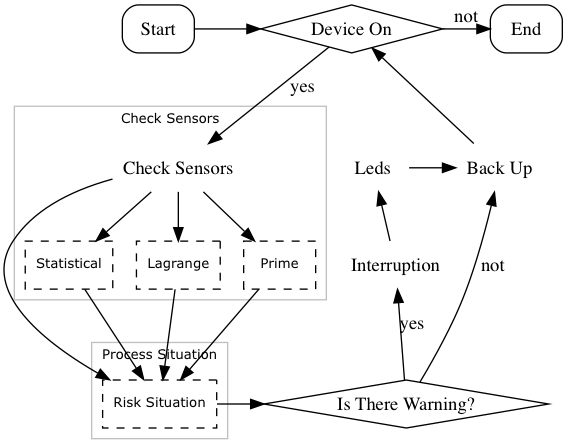
\includegraphics[width=0.45\textwidth]{img/capacete.png}
            \caption{Algorithm call graph of wearable base. Grid items display the location of partitioning algorithms.}
            \label{fig:gc}
        \end{figure}
        
        %O particionamento foi avaliado em duas seções principais, sendo elas a de leitura e de processo de situações, constituindo-se de quatro situações diferentes de particionamento para análise (itens pontilhados na Figura \ref{fig:gc}).
        The partitioning was evaluated in two main sections, mean them the check of distance and situations processing, constituting of four different situations of partitioning for analyzing (items dotted in Figure~\ref{fig:gc}).
        
        %Os algoritmos \A$_{i}$\ candidatos ao particionamento serão:
        The candidate algorithms \A$_{i}$\ to the partitioning was:
        
        \begin{itemize}
            %\item \A$_{St}$: Análise Estatística (Algoritmo \ref{alg:statistic}) calculará valores de desvio padrão e variância dos valores no \buffer;
            \item \A$_{St}$: Statistical Analysis (Algorithm \ref{alg:statistic}) will calculate the standard derivation and variance of the buffer's values;
            
            %\item \A$_{La}$: Lagrange (Algoritmo \ref{alg:lagrange}) interpolará novas distâncias a partir dos dados do \buffer; 
            \item \A$_{La}$: Lagrange (Algorithm \ref{alg:lagrange}) will interpolate new distances by buffer's values;
            
            %\item \A$_{PN}$: Números Primos (Algoritmo \ref{alg:prime}) avaliará se a soma das distâncias lidas correspondem aos números primos;
            \item \A$_{PN}$: Prime Numbers (Algorithm \ref{alg:prime}) will evaluate if the sum of distances read correspond to a prime number;
            
            %\item \A$_{Ri}$: Processamento de risco (Algoritmo \ref{alg:risk}), na seção de processo de situações.
            \item \A$_{Ri}$: Risk Processing (Algorithm \ref{alg:risk}), in section of situation process.
        \end{itemize}
    
    
        %!TEX root = ../main.tex
% !TeX encoding = UTF-8

       \begin{algorithm}[t] \footnotesize
           \KwIn{buffer vector.}
           \KwOut{mean, variance, standard derivation.}
           
           \BlankLine
           \Begin{
               $\vars{sum}= \vars{variance} = 0$;
               \BlankLine
               
               \lFor{$\func{length}(\vars{buffer})$}{$\vars{sum} \mathrel{+}= \vars{buffer}_i$}
               \BlankLine
               
               $\vars{mean} = \vars{sum} \div \func{length}(\vars{buffer})$\;
               \BlankLine
               
               
               \lFor{$\func{length}(\vars{buffer})$}{
                   $\vars{variance} \mathrel{+}= (\vars{buffer}_i - \vars{mean})^2$
               }
               
               \BlankLine
               $\vars{variance} \mathrel{\div}= \func{length}(\vars{buffer})$\;
               \BlankLine
               $\vars{sd} = \func{sqrt}(\vars{variance})$\;
               
               \Return \vars{mean}, \vars{variance}, \vars{sd}\;
           }
           \caption{Statistical Method.}
           \label{alg:statistic}
       \end{algorithm}
       
       \begin{algorithm}[b] \footnotesize
           \KwIn{buffer vector, point.}
           \KwOut{interpolated distance.}
           
           \BlankLine
           \Begin{
               
               $\vars{new\_distance} = 0$\;
               \BlankLine
               
               \For{$\vars{i}\ in\ 1:\func{length}(\vars{buffer})$}{
                   $\vars{c} = \vars{d} = 1$;
                   
                   \BlankLine
                   \For{$\vars{j}\ in\ 1:\func{length}(\vars{buffer})$}{
                       \If{$\vars{i} \ne \vars{j}$}{
                           $\vars{c} \mathrel{\times}= \vars{point} - \vars{j}$;
                           %\BlankLine
                           $\vars{d} \mathrel{\times}= \vars{i} - \vars{j}$;
                       }
                   }
                   \BlankLine
                   $\vars{new\_distance} \mathrel{+}= \vars{buffer}_i \times \vars{c} \div \vars{d}$;
               }
               \BlankLine
               
               \lIf{$\vars{new\_distance} \ge 0$}{$\Return\ \vars{new\_distance}$}
               \lElse{$\Return\ 0$}
               
           }
           \caption{Interpolation by Lagrange Method.}
           \label{alg:lagrange}
       \end{algorithm}
       
       \begin{algorithm}[t] \footnotesize
           \KwIn{distance$_1$, distance$_2 = 0$, distance$_3 = 0$.}
           \KwOut{primacy.}
           
           \BlankLine
           \Begin{
               
               $\vars{prime} = \vars{distance}_1 + \vars{distance}_2 + \vars{distance}_3$;
               \BlankLine
               
               \lIf{$\vars{prime} \le 1$}{\Return 0}
               \BlankLine
               \lIf{$\vars{prime} = 2$}{\Return 1}
               \BlankLine
               
               \lIf{\vars{prime} $\func{mod}(2) = 0$}{$\vars{prime} \mathrel{+}= 1$}
               \BlankLine
               
               $\vars{divider} = \vars{prime} \div 2$;
               
               \lIf{\vars{divider} $\func{mod}(2) = 0$}{$\vars{divider} \mathrel{+}= 1$}
               \BlankLine
               
               
               \While{\vars{divider} $> 2$}{
                   \lIf{\vars{prime} $\func{mod}(divider) = 0$}{\Return 0}
                   \BlankLine
                   \lElse{\vars{divider} $\mathrel{-}= 2$;}
                   
               }
               \Return 1;
               
           }
           \caption{Prime Number Method.}
           \label{alg:prime}
       \end{algorithm}
       
       \begin{algorithm}[b]
           \footnotesize
           \KwIn{distance read; min distance.}
           \KwOut{boolean.}
           
           \BlankLine
           \Begin{
               \tcp{If there is risk, return TRUE}
               \uIf{\vars{distance\_read} $\le$ \vars{min\_distance}}{
                   \Return 1
               }
               \lElse {
                   \Return 0
               }
               
           }
           \caption{Risk Processing Method.}
           \label{alg:risk}
       \end{algorithm}
       
        
        %Explicando as implementações de A
        %Foi realizado o particionamento para cada algoritmo candidato \A$_{i}$, gerando tanto sua versão em código em nível de \software,\ quando seu módulo em \hardware,\ utilizados para testes comparativos de desempenho.
        It was made the partitioning for each candidate algorithm \A$_{i}$, building both its software level code version and its hardware module, both used for comparative tests.
        
        % s de forma geral
        %Para a execução dos testes, todos os \A$ _i $\ em suas versões \hs\ foram executados em implementações sistêmicas sintetizáveis \Ss$ _j $,\ constituídas de módulos como \textit{soft-}processador MicroBlaze, além de memórias, interfaces para comunicação com os dispositivos conectados, entre outros, permitindo o funcionamento completo do \wearable\ \cite{obeidat2011microblaze}.
        For the execution of the tests, all the \A$ _i $\ in its hardware and software versions ran in synthesizable systemic implementations \Ss$ _j $,\ constituted of modules as MicroBlaze soft-processor, beyond of memories, interfaces for communication with the connected devices, among others, allowing the full operation of wearable \cite{obeidat2011microblaze}.
        
        % as versões de a em software
        %Todos os algoritmos \A$_{i}$ em suas versões de \software\ foram executados em uma única implementação \Ss$ _j $, já que esta era compatível com qualquer aplicação em nível de \software, dependendo somente da disposição das instruções na memória.
        %Ou seja, para trocar o \A$_{i}$ por \A$_{k}$ neste sistema basta recompilar o projeto em \software.
        %Os testes neste sistema serão referenciados como \Ss$ _{s} $.
        All the algorithms \A$ _i $\ in its software versions ran in one unique \Ss$ _j $ implementation, since it was compatible with any application in software level, depending only on the availability of instructions in its memory.
        In other words, to change the \A$ _i $ to \A$ _k $ in this system need to recompile the project in software.
        The tests in this system will be referenced as \Ss$ _{s} $.
        
        % algoritmos em hardwares
        % explicando que a necessitam de interfaces
        %Algoritmos \A$ _i $\ em \hardware\ também executam em sistemas \Ss$ _j $, mas tais sistemas possuem características ímpares já que são acrescentados módulos sintetizáveis de cada algoritmo.
        %
        %Como cada \A$_i$ possui seu próprio módulo, definiu-se um sistema \Ss$_j$ para cada algoritmo \A$_{i}$ em sua versão em nível de \hardware.
        Algorithms \A$ _i $\ in hardware also run in \Ss$ _j $ systems, but such systems have unique features as they are added with their synthesizable modules.
        As each \A$ _i $ has its module, we defined a system \Ss$ _j $ for each algorithm \A$ _i $ in its hardware level version.
        
        %Assim, como a Tabela~\ref{tab:bate_o_olho} exibe, \Ss$_s$ é o sistema para testes de todos os algoritmos \A$_{i}$\ em \softwares,\ não possuindo nenhuma adição de implementação sintetizável de \hardwares\ particionados.
        %Os outros sistemas são para testes dos módulos dos respectivos algoritmos \A$ _i $ juntos de sua interface de comunicação \hs.
        So, as the Table~\ref{tab:bate_o_olho} shows, \Ss$ _s $ is the system for the tests of all the algorithms \A$ _i $ in software level, not having any synthesizable implementation of partitioned hardware.
        The others systems are for tests of the modules of the respective algorithms \A$ _i $ with its hardware and software communication interface.
        
        \begin{table}[h]\centering
            \vspace{-1em}
            \scriptsize
            %\raaa{1.0}
            \raaa{0.9}
            \caption{Candidate Algorithms and their Test Systems}

            \begin{tabular}{p{2.3em}p{1.3em}|p{1.3em}p{0.01em}p{1.3em}|p{1.3em}p{0.01em}p{1.3em}|p{1.3em}p{0.01em}p{1.3em}|p{1.3em}}
                \toprule
                & \multicolumn{2}{c}{\A$_{St}$} && \multicolumn{2}{c}{\A$_{La}$} && \multicolumn{2}{c}{\A$_{PN}$} && \multicolumn{2}{c}{\A$_{Ri}$}\\ %\cmidrule{2-9}
                \cmidrule{2-3} \cmidrule{5-6} \cmidrule{8-9} \cmidrule{11-12}
                Impl.: & \textit{Soft.} & \textit{Hard.} && \textit{Soft.} & \textit{Hard.} && \textit{Soft.} & \textit{Hard.} && \textit{Soft.} & \textit{Hard.} \\ \midrule
                \Ss$_{s}$   & X &   && X &   && X &   && X &   \\ \hline
                \Ss$_{St}$  &   & X &&   &   &&   &   &&   &   \\ \hline
                \Ss$_{La}$  &   &   &&   & X &&   &   &&   &   \\ \hline
                \Ss$_{PN}$  &   &   &&   &   &&   & X &&   &   \\ \hline
                \Ss$_{Ri}$  &   &   &&   &   &&   &   &&   & X \\
                \bottomrule
            \end{tabular}
            \label{tab:bate_o_olho}
        \end{table}
        
        
        
        
    \subsubsection{Prototype's Variations}
        %A fim de fazer diferentes testes dos códigos particionados foi construído um protótipo modular para a realização de análises de desempenho sobre cada uma de suas variações.
        %Os itens modulares são:
        To make different tests of partitioned codes a modular prototype was built to carry out performance analyzes on each of its variations.
        The modular items were:
        \begin{itemize}
            %\item Número de Sensores de Distância: testes serão realizados com um a três sensores. 
            %Não aumenta-se a angulação de percepção, mas sim a exatidão dos dados lidos;
            \item The Number of Distance Sensors: tests will be performed with one to three sensors.
            The angulation of perception is not increased, but the accuracy of the data read;
            
            %\item \textit{Buffer} de Cada Sensor de Distância: \buffer\ de dados com tamanho 5, 10 e 15 para processamento das distâncias de cada sensor.
            %Representam a quantidade de leituras que serão feitas para cada sensor, armazenando-as num vetor, na qual será utilizado como parâmetro para as operações que serão particionadas.
            \item Buffer for Each Distance Sensor: data buffer with size 5, 10 and 15 for processing the distances of each sensor.
            They represent the number of readings that will be made for each sensor, storing them in a vector, in which it will be used as parameter for the operations that will be partitioned.
        \end{itemize}
        %Dessa forma, sobre cada código candidato foi realizados testes segundo tais variações, tanto em \hardware,\ quanto em \software.
        In this way, over each candidate code was made tests according to those variations, both in hardware and software.
    
    
    \subsubsection{Equipment and Technologies Used}
        %A placa utilizada para sintetização foi uma Arty A7-35T, com 32 mil \luts\ sem um \textit{hard-processor}, ou seja, um controlador/processador físico dedicado.
        %Para isso, utilizou-se o sistema \textit{soft-processor} MicroBlaze para processamento do código em \software\ e comunicação com \hardware.
        The board used to synthesize was the Arty A7-35T, with 32 thousand LuTs without a hard-processor, that is, a physic controller/processor dedicated.
        To this, we used the MicroBlaze soft-processor system for the software level code processing and communication with the hardware.
        
        
        %Todos os algoritmos foram construídos utilizando-se a ferramenta HLS e incorporados ao projeto base com construções de circuitos digitais assistidos pelo computador.
        %A comunicação entre \hs\ foi feita utilizando interface AXI.
        %A medição de distância foi realizada com um sensor ultrassônico e a comunicação com um segundo dispositivo que utiliza \textit{Bluetooth Low Energy}.
        All the algorithms were built using the HLS tool and integrated to the base project with constructions of digital circuits assisted by the computer.
        Communication between hardware and software was done using AXI interface.
        The distance check was made by the ultrasonic sensor and the communication with a second device was with Bluetooth Low Energy.
        
        
    \subsection{Tests}
        % Explicando os testes
        %Para a realização dos testes foi feito um procedimento, tendo como base a Figura \ref{fig:distance}. 
        %Como o experimento foi realizado em laboratório, utilizou-se escala de centímetros para as análises.
        To the tests was made a procedure, based on the Figure~\ref{fig:distance}.
        As the experiment was done in a laboratory, we used centimeters scale for the analysis.
        
        \begin{figure}[h] \centering
            %\vspace{-0.5em}
            
\includegraphics[width=0.5\textwidth]{img/distance.png}
            \caption{Simulation of approach of objects to the cyclist according to their respective safety areas.}
            \label{fig:distance}
        \end{figure}
    
        %Cada experimento foi realizado no decorrer de 12 iterações.
        %Os principais passos do teste são:
        Each experiment was done in the course of 12 iterations.
        The main steps of the test are:
        \begin{itemize}
            %\item \textit{Iteração 1:} o ciclista, encontra-se a uma distância de 130 centímetros do objeto, sendo sua situação declarada como segura;
            \item Iteration 1: the cyclist, is at a distance of 130 centimeters of the object, and his situation is declared as safe;
            
            %\item \textit{Iteração 4:} o objeto inicia um movimento de aproximação\footnote{Tanto o movimento de aproximação quanto o de afastamento são realizados manualmente por humanos, simulando a situação real de um ciclista em seu meio.} ao ciclista chegando a ultrapassar o limite mínimo de 30 centímetros. Nisso, a situação do ciclista passa a ser de risco;
            \item Iteration 4: the object initiates a movement of approximation\footnote{Both the approximation and the removal movements are performed manually by humans, simulating the actual situation of a cyclist in their environment.} to the cyclist reaching to exceed the minimum limit of 30 centimeters. 
            In this, the situation of the cyclist happens to be of risk;
            
            %\item \textit{Iteração 6:} o objeto ainda encontra-se próximo ao ciclista;
            \item Iteration 6: the object is still close to the cyclist;
            
            %\item  \textit{Iteração 9:} o objeto afasta novamente do ciclista para 130 centímetros, retornando à situação segura;
            \item Iteration 9: the object moves away from the cyclist to 130 centimeters, returning to the safe situation;
            
            %\item  \textit{Iteração 12:} última leitura para testes, ciclista ainda em situação segura.
            \item Iteration 12: last reading for tests, cyclist still in safe situation.
            %
        \end{itemize}
    
        %As iterações não citadas representam a permanência do estado da iteração anterior à ela.
        The non-cited iterations represent the permanence of the state of the iteration prior to it.
   
        %Este teste foi realizado em cada análise de particionamento com sua variação de módulo. 
        %Ou seja, para cada um dos 4 algoritmos, em todas suas variações de sensores e \buffer, um total de 36 situações diferentes para \hs\ serão feitos 30 testes em sequência para cada uma dessas situações, para análises estatísticas de desempenho.
        This test was done in each analyze of partitioning with its module variation.
        That is, for each one of the four algorithms, in all its variations of sensors and buffer in both hardware and software, was done 30 tests in sequence for each situation.
        
        %Como a pesquisa tem o objetivo de avaliar o desempenho dos algoritmos candidatos em \hs,\ os tempos de envio de dados e atuação dos sensores foram descartados.
        As the research has the target to evaluate the performance of candidate algorithms in hardware and software, discarded the send data and sensor's actuation time.
        
        
\section{Results}   \label{chap:results}
    
    \subsection{Allocated Resources for the \A$_{i}$ Algorithms and \Ss$_{j}$ Systems}
        
        % tabela hls
        %Os valores exibidos pela Tabela \ref{tab:hls} quantificam os recursos utilizados pelo HLS para a geração de cada algoritmo \A$_{i}$ particionado em \hardware.
        %
        %Cada linha exibe os valores de alocação referentes a cada algoritmo, sendo os algoritmos Estatístico \A$_{St}$, Lagrange \A$_{La}$, Números Primos \A$_{PN}$ e Risco \A$_{Ri}$.
        %Já as colunas exibem para quais propósitos determinados recursos em \hardware\ foram utilizados, na qual são expressões, instâncias, multiplexadores e registradores.
        %Todos são formados das tecnologias \luts\ e \ffs.       
        %
        %Na última coluna é contabilizado o total de gastos de cada \hardware\ gerado.
        Table~\ref{tab:hls} shows the values quantify the resources used by HLS for the generation of each algorithm \A$ _i $ partitioned in hardware.
        Each line shows the allocation values referent each algorithm, being them Statistical \A$_{St}$, Lagrange \A$_{La}$, Prime Numbers \A$_{PN}$ e Risk \A$_{Ri}$.
        The columns show for which proposes some resources in hardware was used, which are the expression, instances, multiplexes, and registers.
        All they are made by LuTs and Flip-Flops technologies.
        In the last column is shown the among spent in each algorithm generated by HLS.
        
        \begin{table*}[t]\centering
            \vspace{-1em}
            \scriptsize
            %\raaa{1.0}
            \raaa{0.9}
            \caption{FPGA Resources Allocated for Each Partitioned Code Using HLS}
            \begin{tabular}{lrr|rr|rr|rr|rr}
                \toprule
                &\multicolumn{2}{c}{Expressions} & \multicolumn{2}{c}{Instances}      & \multicolumn{2}{c}{Multiplexes}  & \multicolumn{2}{c}{Registers} & \multicolumn{2}{c}{\textit{Total}} \\
                \cmidrule{2-11}
                %\cmidrule{2-3} \cmidrule{5-6} \cmidrule{8-9} \cmidrule{11-12} \cmidrule{14-15}
                & \luts & \ffs & \luts & \ffs & \luts & \ffs & \luts & \ffs & \luts & \ffs \\
                \midrule
                \A$_{St}$&52 & 0     & 1948 & 1474   & 364 & 0      & 0 & 394   & 2364 & 1868 \\ 
                \A$_{La}$&128 & 0    & 2048 & 1425   & 309 & 0      & 0 & 479   & 2483 & 1904 \\ 
                \A$_{PN}$&1826 & 0   & 486 & 552     & 236 & 0      & 0 & 527   & 2448 & 1079 \\ 
                \A$_{Ri}$&18 & 0     & 120  & 82     & 15  & 0      & 0 & 34    & 153  & 116  \\ 
                \bottomrule
            \end{tabular}
            \label{tab:hls}
        \end{table*}
        
        %Linkando a com b
        %Com cada o módulo particionado gerado, deve-se então adicioná-los aos respectivos sistemas.
        
        
        
        %\subsubsection{Recursos Para Cada Sistema \Ss}
        %Exibido os valores para cada \A$ _i $,\ a Tabela~\ref{tab:vivado} mostra os valores de alocação e gasto energético sobre cada sistema \Ss$_{j}$ utilizado para teste.
        %As colunas exibem informações de alocação de \luts, \ffs\ e \luts RAM e o gasto energético médio (\textit{Chip Power}) de cada um dos sistemas \wearables\ testados no protótipo.
        %A primeira linha exibe a quantidade de cada recurso disponível pela plataforma FPGA utilizada e as demais o valor alocado segundo cada sistema.
        Shown the values for each \A$ _i $,\ the Table~\ref{tab:vivado} shows the allocation and energy spent amounts in each \Ss$_{j}$\ system used for the test.
        The columns show information of LuTs, LuTRAMs and Flip-Flop allocations and energy cost mean (Chip Power).
        The first line shows the number of available resources in the FPGA platform used and the rest the allocated value according to each system.
        
        \begin{table}[t]\centering
            \vspace{-1em}
            %\scriptsize
            \footnotesize 
            %\raaa{1.0}
            \raaa{0.9}
            \caption{Resources and Energy Cost Used in All Complete Systems}
            \begin{tabular}{lcccc}
                \toprule
                & \lut   & Lu.T.\textit{RAM} & \ff             & \textit{Chip Power} \\
                \cmidrule{2-5}
                
                \textit{Available}& \textit{20800}  & \textit{9600}              & \textit{210}     & -      \\\cmidrule{1-5}
                \Ss$_{s}$ & 11991  & 1781              & 11612           & 0,922W \\
                \Ss$_{St}$& 13640  & 1822              & 13080           & 0,972W \\ 
                \Ss$_{La}$& 13502  & 1808              & 13193           & 0,968W \\ 
                \Ss$_{PN}$& 12959  & 1782              & 12559           & 0,933W \\
                \Ss$_{Ri}$& 12109  & 1781              & 11742           & 0,929W \\ 
                \bottomrule
            \end{tabular}
            \label{tab:vivado}
        \end{table}
    
        %Com esses valores é possível fazer análises de recursos utilizados tanto para os módulos de maneira isolada, quanto para o sistema como um todo.
        %Assim, percebeu-se que:
        With these values, it is possible to analyze resources used for both the modules isolated and for the all system as well.
        So, we analyzed that:


   %\subsection{Análise sobre Quantidade de Recursos Alocados e Gasto Energético}
        %Analisando as Tabelas~\ref{tab:hls} e \ref{tab:vivado}, é possível ver que:
        
        \begin{itemize}
            \item 
            % codigo que gastou mais recurso
            %\A$_{La}$ é o módulo particionado que utiliza mais recursos dentre todos.
            %Mesmo assim, ao incorporar os códigos particionados aos sistemas, seu sistema (\Ss$_{La}$) não é o maior em utilização de recursos;
            \A$_{La}$ is the partitioned module that uses more resources than everyone else.
            Even so, incorporating the partitioned codes into the systems, its \Ss$_{La}$ system is not the biggest in resources utilization;
            
            \item
            %sistema que mais gastou recursos
            %Ainda sobre a utilização de recursos, a maior diferença entre sistemas completos (particionados com o sistema em \software)\ é de $5,5\%$, entre \Ss$_{s}$ e \Ss$_{St}$. 
            %Isso pois, enquanto o \Ss$_{s}$ utilizou $45,3\%$ do total de \luts\ disponíveis (ambas \luts\ e \luts RAM), \Ss$_{St}$ utilizou $50,8\%$.
            The most difference between complete systems (partitioned system against the software system) is 5,5\%, between \Ss$_{s}$ and \Ss$_{St}$. 
            That is, while the \Ss$_{s}$ used 45,4\% of total of available LuTs (both LuTs and LuTRAMs), \Ss$_{St}$ used 50,8\%.
            
            
            %Essa diferença entre recursos alocados também está presente na forma em que a interface de comunicação está sendo utilizada em seus módulos.
            %Mesmo \A$_{St}$ não sendo o maior módulo, seu sistema \Ss$_{St}$ foi, indicando que sua interface requisitou grande quantia de recursos;
            This difference between allocated resources also is presents in the way that its modules are using communication interface;
            
            \item
            %Comparando o gasto energético dos sistemas particionados com o sistema em \software, o maior gasto também é de \Ss$_{St}$, necessitando de $5,4\%$ W a mais que \Ss$_{s}$. \\
            Comparing the energy spent of partitioned and software systems, the most significant cost \Ss$_{St}$, needing 5,4\% Watts more than \Ss$_{s}$.
            
            %O sistema com o módulo Lagrange em \hardware\ (\Ss$_{La}$) teve a menor diferença, utilizando $0,7\%$ Watts a mais que \Ss$_{s}$.
            The Lagrange module with its system (\Ss$_{La}$) had the smallest difference, using 0,7\% Watts more than \Ss$ _s $.
        \end{itemize}
           
           

    \subsection{Performance}
    
        %A Figura \ref{fig:performance} exibe os valores obtidos das análise de desempenho entre \hs\ (conforme apresentado na Seção \ref{sec:ganho_performance}).
        %Mostra-se todos os algoritmos separados em quadros, bem como suas variações de sensores e \buffer.
        The Figure~\ref{fig:performance} shows the values obtained from the performance analysis between hardware and software (according to Section~\ref{sec:ganho_performance}).
        It shows all the algorithms by frames, as well as its buffer and sensors variations.
        
        %No eixo das abscissas tem-se \textit{Sen} e \textit{Buf} representando a variação de sensores e do tamanho de \buffer\ no protótipo.
        %Já no eixo das ordenadas exibe-se o valor performático dos 30 testes para cada uma das 36 situações, segundo a Equação~\ref{eq:speedup1}.
        In the axis of the abscissae we have \textit{Sen} and \textit{Buf} representing the sensors and buffer variations in the prototype.
        At ordinates axis is shown the performance value of the 30 test for each one of the 36 situations, according to Equation~\ref{eq:speedup1}.
        
        \begin{figure*}[h] \centering
            \vspace{-0.5em}
            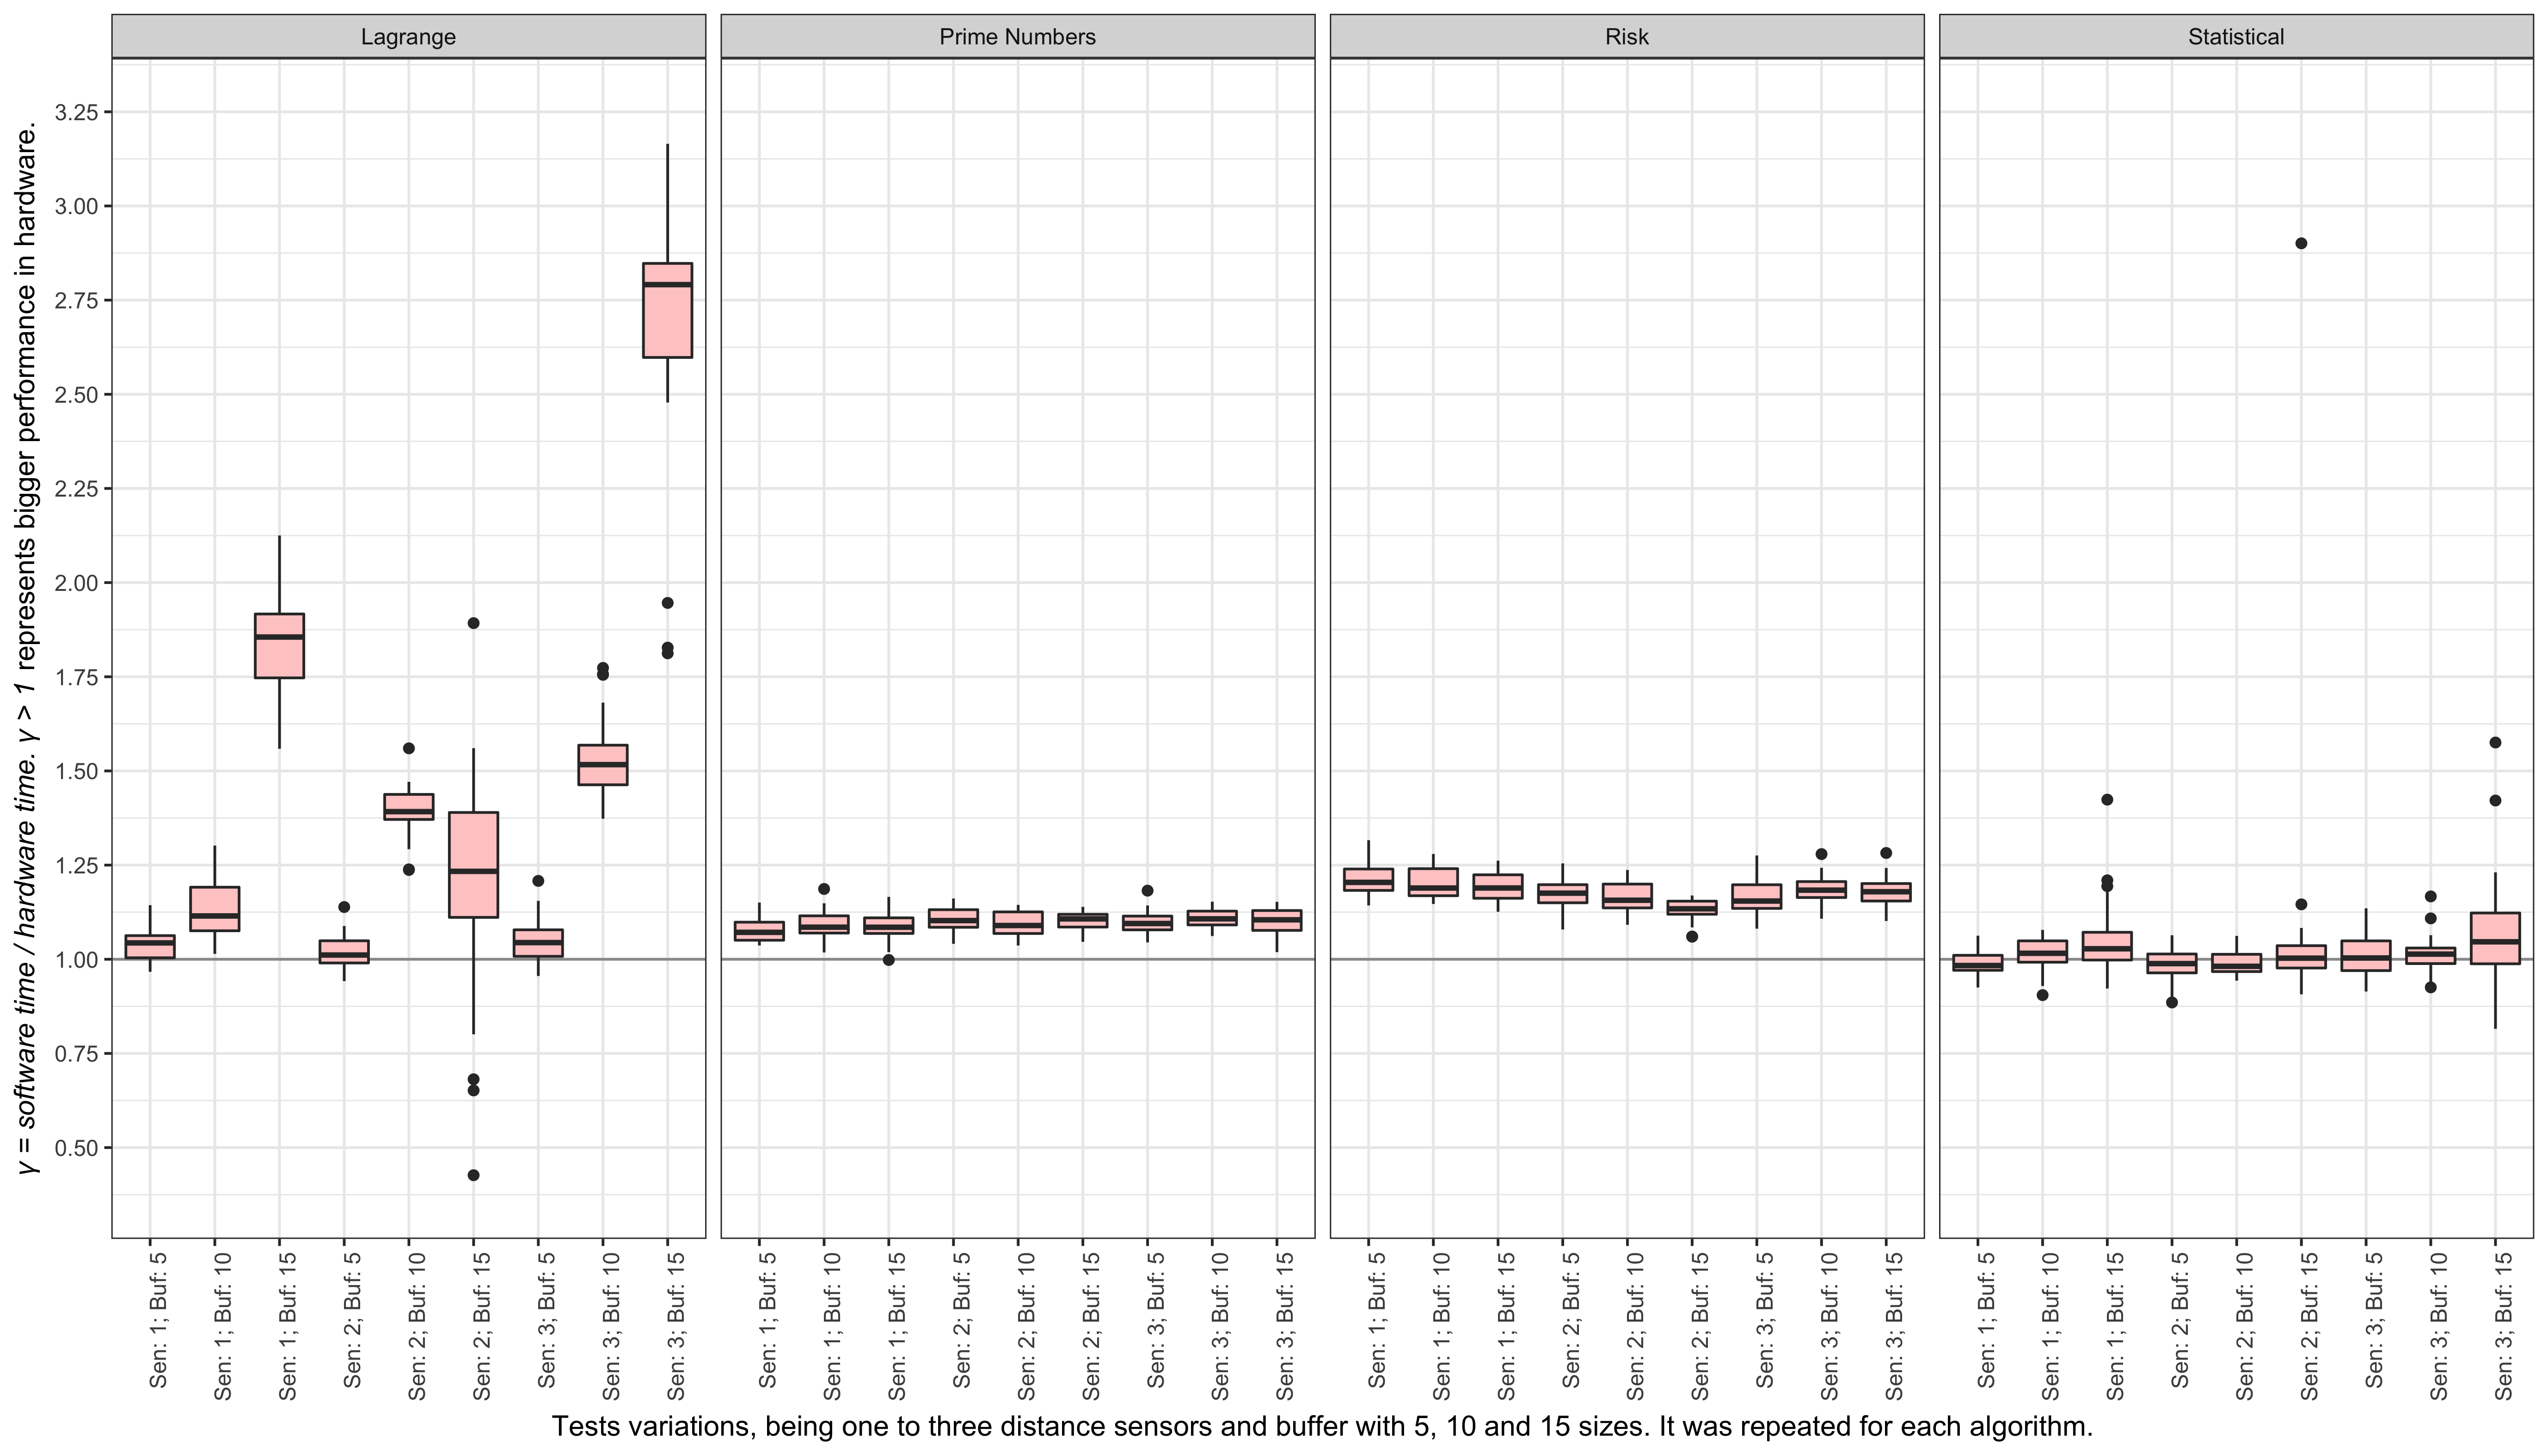
\includegraphics[width=1\textwidth]{img/performance.png}
            \caption{Graphic with the performance values of the 36 prototype variations, separated by candidate code. The values of $ \gamma > 1.0 $ show bigger performance in partitioned hardware than software.}
            
            \label{fig:performance}
        \end{figure*}
   
    
        %Além da Figura~\ref{fig:performance}, os valores médios também podem ser lidos pela Tabela~\ref{tab:performance}.
        %Cada linha desta representa um quadro da Figura~\ref{fig:performance}.
        %Como complemento, na última coluna tem-se uma média de desempenho de cada algoritmo em todas as suas variações de teste.
        Beyond the Figure~\ref{fig:performance}, the mean values also are shown by Table~\ref{tab:performance}.
        Each line represents a frame of Figure~\ref{fig:performance}.
        As a compliment, in the last column has a performance mean of each algorithm in all its test variations.
        
        \begin{table}[b]\centering
            \vspace{-1em}
            \scriptsize
            \raaa{1.0}
            %\raaa{0.9}
            \caption{Mean of Performance Analysis in its Variations}
            \begin{tabular}{@{}R{1.3em}R{1.6em}R{1.5em}R{1.5em}|R{1.6em}R{1.6em}R{1.6em}|R{1.5em}R{1.5em}R{1.5em}|c@{}}\toprule
                & \multicolumn{3}{c}{1 Sensor} & \multicolumn{3}{c}{2 Sensors} & \multicolumn{3}{c}{3 Sensors}& \\
                \cmidrule{2-11}
                \textit{Buffer} & 5 & 10 & 15 & 5 & 10 & 15 & 5 & 10 & 15 & $\bar{x}$ \\
                \midrule
                \Ss$_{St}$   & 0.989 & 1.013 & 1.052  & 0.982 & 0.992 & 1.069  & 1.009 & 1.011 & 1.08  & 1.022 \\
                \Ss$_{La}$   & 1.036 & 1.132 & 1.844  & 1.019 & 1.395 & 1.14   & 1.046 & 1.37  & 2.765 & 1.416 \\
                \Ss$_{PN}$   & 1.076 & 1.092 & 1.084  & 1.105 & 1.094 & 1.103  & 1.099 & 1.109 & 1.102 & 1.096 \\ 
                \Ss$_{Ri}$   & 1.212 & 1.203 & 1.195  & 1.17  & 1.161 & 1.132  & 1.168 & 1.183 & 1.179 & 1.178 \\
                \bottomrule
            \end{tabular}
            \label{tab:performance}
        \end{table}
        
        %Análise de performance
        % quase todos foram suuuuuuuucesssooooooooo 
        %Os resultados mostram que:
        The results show that:
        \begin{itemize}
            \item 
            %Os algoritmos Número Primo e Risco (\Ss$_{PN}$ e \Ss$_{Ri}$) obtiveram um ganho de desempenho considerável e estável, comparado com suas versões não particionadas, sendo em média $9,6\%$ e $17,8\%$ mais eficiente em suas tarefas;
            The Prime Number and Risk Algorithms (\Ss$_{PN}$ and \Ss$_{Ri}$) have a considerable and stable performance gain comparing with its versions non-partitioned, being meanly 9,6\% and 17,8\% more efficient in its tasks;
            
            \item 
            %Mesmo com o algoritmo Lagrange (\Ss$_{La}$) exibindo resultados não-estáveis nas variações como os de \Ss$_{PN}$ e \Ss$_{Ri}$, $87\%$ dos testes realizados obtiveram maior desempenho em \hardware.
            %Superando a versão em \software\ em $41,6\%$;
            Even with the Lagrange (\Ss$_{La}$) showing results not so stables in its variations as the \Ss$_{PN}$ and \Ss$_{Ri}$, 87\% of its tests had bigger performance in hardware.
            It overcame its software version in 41,6\%;
            
            \item 
            %O algoritmo Estatístico (\Ss$_{St}$) obteve três situações, na qual não utilizar o particionamento resultava em maior desempenho, sendo $45,5\%$ foram iguais ou melhores em \software.
            %São elas: [\textit{Sen} 1; \textit{Buf} 5], [\textit{Sen} 2; \textit{Buf} 5] e [\textit{Sen} 2; \textit{Buf} 10]. 
            %Entretanto, a média de todos os seus testes mostram que ainda assim foi $2,2\%$ mais eficiente em \hardware\ que \software.
            The Statistical (\Ss$_{St}$) obtained three situations, in which not using partitioning resulted in higher performance, being 45,5\% was equal or bigger in software.
            Are they: [\textit{Sen} 1; \textit{Buf} 5], [\textit{Sen} 2; \textit{Buf} 5] and [\textit{Sen} 2; \textit{Buf} 10]. 
            However, the mean of all its tests shows that they still were 2,2\% more efficient in hardware than software.
        \end{itemize}
    
    
        %\item 
        % Achismos
        %O baixo resultado de \Ss$_{St}$ já era esperado, pois este e todos os outros algoritmos não receberam nenhuma otimização em \hardware,\ nem em sua interface de comunicação.
        %O algoritmo Estático especificamente (Algoritmo \ref{alg:statistic}), é o único que realiza mais de uma leitura sobre os dados de \buffer\ via parâmetro, sendo as operações situadas nas linhas 3 e 5.
        %Este algoritmo é custoso, pois o uso de cada elemento de \buffer\ requer também uma comunicação entre \hs,\ solicitando o respectivo dado, criando uma sobrecarga no barramento e, consequentemente, a queda de desempenho pela sua espera.
        The low result of \Ss$_{St}$ was already expected because this and all the others algorithms neither received optimizations in hardware nor communications interface. 
        The \Ss$_{St}$ is explicitly the only that does more than one read over the buffer data via parameter, being the operations in lines 3 and 5 of Algorithm \ref{alg:statistic}.
        This algorithm is expensive, because the use of each buffer element also requires a hardware and software communication, requesting the respective data, making an overload and consequently, the performance decline.
        
        
        %resolvendo o problema
        %Este problema pode ser contornado de várias formas.
        %A mais simples seria utilizar uma memória interna no \hardware\ extra que, após a cópia de todos os valores do \buffer, pode-se operar lendo da sua própria memória.
        %\textit{Pipeline}, \textit{unroll} de \textit{loops} e protocolos de comunicação adequados são tipos de otimizações mais complexas, mas que poderiam resultar em melhora de desempenho, não aplicando só ao Estatístico, mas também todos os outros.
        This problem can be resolved in many ways.
        The most simple would be to use an internal memory in hardware that, after the copy, the buffer data to it, can operate reading of its memory.
        A pipeline, unroll loops, and better communications protocols also are types of optimizations more complexes, but that could result in performance enhancement, not applying just for Statistical, but all of the rest.
        

%!TEX root = ../main.tex
% !TeX encoding = UTF-8
\section{Conclusions} \label{chap:conclu}
    %projeto de sistemas
    %A demanda por curto tempo para disponibilidade ao mercado, somado ao fato dos produtos exigirem propriedades de corretude, rapidez, confiabilidade e preço acessível representam um desafio para projetistas de sistemas embarcados em geral.
    %utiliza o particionamento para o problema de desempenho
    %Com o desenvolvimento de sistemas embarcados cada vez mais complexos, o particionamento \hs\ tornou-se um problema de otimização em \codesign\ de sistemas.
    %wearable
    %Como dispositivos \wearables\ também demandam um alto desempenho e/ou baixo consumo de energia sem apresentar desequilíbrio em confiabilidade e segurança entre outros, aplicou-se o particionamento sobre essa classe de sistemas, com foco em tais melhorias.
    The short time demand for market disponibility summed up to the fact of products requires correctness, speed, reliability and affordable price proprieties represent a challenge for ES designers in general.
    With the ES development is increasingly complex, the hardware and software partitioning became an optimization problem in systems codesign.
    As wearable devices also require high performance and low energy cost without the tradeoff, was applied the partitioning in this system class targeting those improvements.
    
    %proposta
    %A proposta da pesquisa constituiu-se na busca pelo aprimoramento de desempenho de dispositivos computacionais \wearables,\ utilizando o particionamento como meio, visando gasto energético e de recursos limitados de plataforma FPGA.
    The propose of this research is to reach the enhancement of performance of wearable devices, using the partitioning, aiming energy spent and limited resources of FPGA platform.
    
    
    %comentando os testes
    %Para a avaliação, realizou-se particionamento de quatro algoritmos candidatos (Estatístico \A$_{St}$, Lagrange \A$_{La}$, Números Primos  \A$_{NP}$ e Processamento de Risco \A$_{Ri}$) de um projeto de capacete de segurança para ciclistas, variando cada teste em quantidade de sensores e também o \buffer\ de operação.
    For the evaluation, we partitioned four candidate algorithms (Statistical \A$_{St}$, Lagrange \A$_{La}$, Prime Numbers  \A$_{NP}$ and Risk Processing \A$_{Ri}$) of a helmet design for safety for cyclists, varying each test in sensors numbers and buffer size.
    
    % comentando os resultados
    %Três dos quatro sistemas (Lagrange \Ss$_{La}$, Números Primos \Ss$_{NP}$ e Risco \Ss$_{Ri}$) obtiveram sucesso na busca por desempenho apenas pelo processo de particionamento, aumentando no mínimo $9,6\%$ seus desempenhos, utilizando o valor máximo de $ 5,5\% $ de recursos e $ 5,4\% $ de energia do \hardware\ reconfigurável.
    %
    %O sistema Estatístico \Ss$_{St}$ em $45,5\%$ dos testes obteve maior desempenho \software\ comparado com \hardware.
    %Esse resultado já era esperado, já que seu código exige bastante comunicação entre \hs, afetando seu desempenho.
    Three of four systems (Lagrange \A$_{La}$, Prime Numbers  \A$_{NP}$ and Risk Processing \A$_{Ri}$) had success in reach for performance only by partitioning process, increasing at least 9,6\% of performance, using the maximum value of 5,5\% of resources and 5,4\% of the energy of reconfigurable hardware.
    The Statistical \Ss$_{St}$ in 45,5\% of tests had bigger performance in software than hardware.
    This result was already expected since its code requires more hardware and software communication, affecting its performance.

    %trabalhos futuros
    %har e softprocessadores
    %Para futuros trabalhos seria possível realizar a comparação do sistema \wearable\ particionado variando, também a arquitetura de sintetização, ou seja, testes de desempenho entre \textit{soft} e \textit{hard-}processadores, ambos utilizando FPGA.
    For future works we would compare the partitioned wearable system also varying its architecture, that is, comparing the wearable performance between soft and hard-processor, both in FPGA platform.
    
    % fpga e prototipações
    %Comparações entre o uso de plataformas FPGA e plataformas de prototipações também seriam viáveis, ainda com foco em busca em otimizações em desempenho e eficiência energética sobre \wearables.
    
    %mais alguma sugestão de trabalhos?
    %E também a adição do parâmetro otimização em \hardware,\ verificando o percentual de ganho ao utilizar as técnicas de otimizações em nível de \hardware\ existentes para HLS.
    
    
    % use section* for acknowledgment
    \section*{Acknowledgment}
        %Agradecemos à Universidade Federal de Ouro Preto, ao CNPq, CAPES e à FAPEMIG pelo subsídio dessa pesquisa.    
        We thank to the Federal University of Ouro Preto, to CNPq, CAPES ant the FAPEMIG by the subsidy of this research.

   % conference papers do not normally have an appendix
   %\section*{Apêndice}    
   %    \hphantom{a}


%\section*{Referências}

%\begingroup
%\renewcommand{\section}[2]{}
% can use a bibliography generated by BibTeX as a .bbl file
% BibTeX documentation can be easily obtained at:
% http://mirror.ctan.org/biblio/bibtex/contrib/doc/
% The IEEEtran BibTeX style support page is at:
% http://www.michaelshell.org/tex/ieeetran/bibtex/
\bibliographystyle{IEEEtran}
% argument is your BibTeX string definitions and bibliography database(s)
%\bibliography{bibliography}
\bibliography{IEEEabrv,bibliography}

%\endgroup

\end{document}
